\documentclass[12pt,a4paper]{article}

% -------------------------------------------------
% Codificación e idioma
% -------------------------------------------------
\usepackage[T1]{fontenc}
\usepackage[utf8]{inputenc}
\usepackage[english,spanish,es-tabla,es-nodecimaldot]{babel}

% -------------------------------------------------
% Página y tipografía
% -------------------------------------------------
\usepackage[a4paper,left=2cm,right=2cm,top=2.25cm,bottom=2.25cm]{geometry}
\usepackage{microtype}
\usepackage{newtxtext,newtxmath} % Times-like, más estable que mezclar con cmbright

% -------------------------------------------------
% Matemáticas y unidades
% -------------------------------------------------
\usepackage{mathtools}
\usepackage{amsmath}
%\usepackage{amssymb}
\usepackage{physics}
\usepackage{siunitx}

\sisetup{
  output-decimal-marker = {.},
  exponent-mode         = threshold,
  exponent-thresholds   = -4:5,
  round-mode            = uncertainty,
  round-precision       = 2,
  print-unity-mantissa  = false,
  inter-unit-product    = \ensuremath{{}\cdot{}},
  inline-per-mode       = single-symbol,
  display-per-mode      = fraction,
  separate-uncertainty = true
}

% -------------------------------------------------
% Figuras y tablas
% -------------------------------------------------
\usepackage{graphicx}
\usepackage{booktabs}
\usepackage{caption}
\captionsetup{
  font=small,
  justification=centerlast,
  skip=6pt,
  labelfont={bf,small},
  textfont={small}
}

% -------------------------------------------------
% Colores e hipervínculos
% -------------------------------------------------
\usepackage[dvipsnames]{xcolor}
\usepackage{hyperref}
\hypersetup{
  colorlinks=true,
  linkcolor=Blue,
  citecolor=ForestGreen,
  urlcolor=BrickRed,
  pdftitle={Centelleo en mezclas gaseosas Ar--CF4 y He--CF4},
  pdfauthor={Daniel Vázquez Lago}
}

% -------------------------------------------------
% Bibliografía
% -------------------------------------------------
\usepackage{csquotes}
\usepackage[
  backend=biber,
  style=numeric,
  sorting=none
]{biblatex}
\addbibresource{sample.bib}

% ------------------------------------------------
% Encabezados y pies
% -------------------------------------------------
\usepackage{fancyhdr}
\pagestyle{fancy}
\fancyhf{}
\fancyhead[L]{Trabajo de Fin de Máster}
\fancyhead[R]{Daniel Vázquez Lago}
\fancyfoot[R]{\thepage}
\renewcommand{\headrulewidth}{0.4pt}
\renewcommand{\footrulewidth}{0pt}


% -------------------------------------------------
% Rutas de figuras
% -------------------------------------------------
\graphicspath{
  {experimental_espectra/}
  {cross_sections/}
  {kinetic_models/}
  {garfield++/}
  {primary_fit/}
  {secondary_fit/}
  {primary_fit_IR_ArCF4/}
  {prediction_plots/}
  {spectra/}
}

\renewcommand{\arraystretch}{1.40}
% -------------------------------------------------
% Macros matemáticas
% -------------------------------------------------
\newcommand{\N}{\mathrm{N}}
\newcommand{\He}{\mathrm{He}}
\newcommand{\Ar}{\mathrm{Ar}}
\newcommand{\CF}{\mathrm{CF}}
\newcommand{\NC}{\mathrm{N}_2^*(\mathrm{C})}
\newcommand{\norma}{\mathrm{norm}}
\newcommand{\vis}{\mathrm{vis}}
\newcommand{\uv}{\mathrm{uv}}
\newcommand{\third}{\mathrm{3rd}}
\newcommand{\dir}{\mathrm{dir}}
\newcommand{\phe}{\mathrm{ph/e^-}}
\newcommand{\vib}{\mathrm{v}}
\newcommand{\nm}{\mathrm{nm}}
\newcommand{\threshold}{\mathrm{threshold}}
\newcommand{\scint}{\mathrm{scint}}

% Versiones robustas para títulos
\DeclareRobustCommand{\Nt}{\ensuremath{\mathrm{N}_2}}
\DeclareRobustCommand{\CFt}{\ensuremath{\mathrm{CF}_4}}
\DeclareRobustCommand{\Argas}{\ensuremath{\mathrm{Ar}}}
\DeclareRobustCommand{\ArCF}{\ensuremath{\mathrm{Ar}-\mathrm{CF}_4}}

% Estados útiles para evitar Unicode raro tipo ¹s4
\DeclareRobustCommand{\ArOneSFour}{\ensuremath{\mathrm{Ar}^*(1s_4)}}
\DeclareRobustCommand{\ArOneSFive}{\ensuremath{\mathrm{Ar}^*(1s_5)}}

% -------------------------------------------------
% Documento
% -------------------------------------------------
\begin{document}
\selectlanguage{spanish}

% -------------------------
% Portada
% -------------------------
\thispagestyle{empty}
\begin{titlepage}
    \centering
    \vspace*{0.20\textheight}

    {\Huge\bfseries Trabajo de Fin de Máster\par}
    \vspace{2.2em}

    {\LARGE\bfseries Centelleo en Mezclas Gaseosas $\Ar-\CF_4$ y $\He-\CF_4$\par}
    \vspace{5em}

    {\Large Daniel Vázquez Lago\par}
    \vspace{2.2em}

    {\Large \today\par}
\end{titlepage}

% -------------------------
% Índice
% -------------------------
\pagestyle{empty}
\tableofcontents
\clearpage

% -------------------------------------------------
% Formato de párrafo
% -------------------------------------------------
\setlength{\parindent}{0pt}
\setlength{\parskip}{0.45em}

\pagestyle{fancy}

\section{Introducción}

La detección de partículas es uno de los pilares experimentales de la física moderna. La información física de un proceso microscópico no se obtiene de forma directa, sino a través de las huellas que dejan las partículas al atravesar la materia: ionización, excitación, centelleo, desplazamiento de carga, producción de calor o emisión de radiación secundaria. En función de cuál de estos observables se quiera privilegiar, y de las condiciones experimentales de cada problema, se han desarrollado familias de detectores muy distintas entre sí. Los detectores de silicio dominan hoy en día los entornos de muy alta ocupación y gran resolución espacial; los calorímetros permiten medir energía y topología de chorros o cascadas; y los detectores basados en gases y en medios nobles continúan siendo una solución especialmente competitiva cuando se buscan grandes volúmenes activos, baja masa material, buena capacidad de imagen y costes razonables por unidad de superficie. En este panorama, el estado del arte no está marcado por una única tecnología, sino por la convivencia de soluciones muy especializadas, optimizadas para necesidades instrumentales diferentes.

\subsection{Detectores Gaseosos}

Dentro de ese ecosistema, los detectores gaseosos mantienen una posición singular. Su principio de funcionamiento es conceptualmente simple: una partícula cargada o una radiación ionizante deposita energía en el gas, crea pares electrón--ión y estados excitados, y la señal se forma a partir del transporte de esas cargas o de la luz emitida durante la excitación y la avalancha. Sin embargo, detrás de esa idea sencilla hay una enorme riqueza instrumental. La composición del gas, la presión, la geometría del detector y el campo eléctrico permiten modular de manera fina la deriva, la difusión, la ganancia, la tasa de \textit{attachment} y la producción de luz. Por ello, los detectores gaseosos siguen siendo una herramienta de referencia en trazado, identificación de partículas, física de neutrinos, búsquedas de procesos raros y detectores de gran volumen 
\cite{gonzlezdaz2017gaseous,hayrapetyan2024dune,next2014present,esfahani2023project}.

En términos históricos, la evolución de los detectores gaseosos puede leerse como una transición desde geometrías macroscópicas, como cámaras de hilos o cámaras proporcionales, hacia estructuras de multiplicación cada vez más finas y controladas. Esa evolución ha respondido a una necesidad muy concreta: reducir la longitud característica de la avalancha para mejorar estabilidad, granularidad, tasa soportada y resolución espacial. En ese contexto aparecen los \emph{micro-pattern gaseous detectors} (MPGDs), que constituyen una de las familias más influyentes en la instrumentación gaseosa contemporánea \cite{shekhtman2002micropattern,buzulutskov2007radiation}. Su importancia no reside solo en haber sustituido en muchos contextos a tecnologías anteriores, sino en haber abierto una vía completamente nueva para combinar multiplicación electrónica, imagen fina y, cada vez más, lectura óptica.

Los MPGDs agrupan dispositivos en los que la amplificación tiene lugar en microestructuras fabricadas con gran precisión: agujeros, mallas o patrones metálicos con dimensiones submilimétricas. Entre los ejemplos más conocidos están los GEM y sus variantes gruesas, como los THGEM, así como otros multiplicadores microestructurados desarrollados para operar en rangos de presión, ganancia o robustez distintos. La ventaja fundamental de estas geometrías es que concentran campos eléctricos intensos en regiones muy pequeñas y bien definidas. Como consecuencia, la avalancha queda más localizada, la respuesta resulta más uniforme, la probabilidad de descarga se controla mejor y la granularidad espacial mejora de manera notable respecto a detectores gaseosos más clásicos \cite{shekhtman2002micropattern,buzulutskov2007radiation,azevedo2016thgem}. Además, la fabricación modular y planar de muchos MPGDs facilita su escalado a áreas grandes y su integración con electrónica segmentada o con sistemas ópticos de lectura.

Desde el punto de vista instrumental, los beneficios de los MPGDs son especialmente atractivos en tres frentes. En primer lugar, permiten trabajar con altas tasas y con patrones de señal muy localizados, algo esencial en experimentos con mucha ocupación o cuando se persigue reconstrucción fina de topologías. Este punto no es solo una ventaja genérica de laboratorio, sino una de las razones por las que los MPGDs han sido adoptados en detectores reales de gran escala. Los GEM de COMPASS demostraron que podían funcionar como trazadores precisos en regiones de alto flujo de partículas; la actualización de la TPC de ALICE sustituyó la lectura proporcional clásica por pilas de GEM para hacer posible la operación en lectura continua a las tasas de interacción de Run 3 y Run 4; y el sistema New Small Wheel de ATLAS emplea Micromegas resistivos en una zona de alto fondo radiativo para proporcionar trazado de precisión y capacidad de disparo en el espectrómetro de muones \cite{ketzer2004compass,adolfsson2021alice,manthos2019atlas}. Estos ejemplos muestran que los MPGDs no son únicamente una tecnología prometedora, sino una solución madura allí donde se necesita combinar granularidad, estabilidad y operación a alta tasa. En segundo lugar, ofrecen una gran versatilidad en la elección de la mezcla gaseosa y de la geometría, lo que permite adaptar el detector a objetivos muy distintos: máxima ganancia, mínima difusión, centelleo intenso o buena resolución temporal. En tercer lugar, los MPGDs son compatibles de forma natural con una lectura híbrida, en la que la misma avalancha puede observarse simultáneamente como carga y como luz. Esa dualidad es una de las razones por las que han pasado de ser simples multiplicadores de carga a convertirse en plataformas muy versátiles para TPCs ópticos, detectores de electroluminiscencia y conceptos avanzados de reconstrucción 3D \cite{oliveira2012simulation,williams2024fatgems}.

\subsection{Centelleo en Detectores Gaseosos}

La utilización del centelleo en MPGDs responde precisamente a esa idea: aprovechar que la avalancha no solo multiplica electrones, sino que también excita especies atómicas y moleculares capaces de emitir fotones. La señal óptica ofrece ventajas que no son redundantes respecto a la carga. En primer lugar, desacopla parcialmente la etapa de amplificación de la de lectura: la información puede recogerse con cámaras, PMTs o SiPMs situados fuera de la zona de alto campo, reduciendo restricciones de cableado y capacitancia. En segundo lugar, la imagen óptica puede proporcionar una granularidad muy alta sobre áreas extensas, especialmente cuando se emplean sensores bidimensionales. En tercer lugar, la luz integra de forma natural información espacial, temporal y topológica: combinada con el tiempo de deriva o con sensores rápidos, permite reconstruir trazas, distinguir morfologías y, en ciertos casos, extraer \emph{timing} absoluto o relativo. Finalmente, en mezclas adecuadas, la emisión puede desplazarse desde el VUV (\textit{Vacuum Ultraviolet}) hacia el UV cercano, el visible o incluso el NIR, regiones donde la fotodetección es tecnológicamente más sencilla y a menudo más barata \cite{bondara2010direct,morozov2012secondary,oliveira2012simulation,santorelli2021spectroscopic,bondar2012study}.

Naturalmente, la lectura por centelleo también introduce limitaciones. La eficiencia óptica total depende no solo del gas, sino de la geometría, del ángulo sólido, de la reflectividad, de las ventanas ópticas y de la eficiencia cuántica o PDE del fotosensor. A diferencia de la carga, la luz puede sufrir pérdidas geométricas importantes y exige una calibración más completa del sistema de detección. Además, la producción de fotones compite con canales no radiativos, con fenómenos de \emph{quenching} colisional y, en determinados gases, con procesos de attachment o de disociación que pueden degradar la linealidad o la estabilidad. En operación a ganancia alta también pueden aparecer efectos de saturación local y de carga espacial en los canales de multiplicación, particularmente relevantes cuando se busca maximizar la salida óptica \cite{christophorou1999electron,amedo2023observation}. En otras palabras, el centelleo en MPGDs no sustituye sin más a la lectura de carga: la complementa, y en algunos escenarios concretos la supera claramente.

A pesar de su interés instrumental, la predicción cuantitativa del centelleo gaseoso sigue siendo un problema mucho menos cerrado que el transporte de carga. Para algunas situaciones concretas sí existen programas experimentales y modelos relativamente desarrollados. Un ejemplo importante procede de la física de rayos cósmicos ultraenergéticos, donde colaboraciones como MACFLY y AIRFLY midieron el rendimiento de fluorescencia de aire seco y N$_2$ puro, así como su dependencia con presión, temperatura, humedad y quenching colisional, con el objetivo de reconstruir la energía de cascadas atmosféricas \cite{colin2007macfly,ave2008airfly}. Sin embargo, ese tipo de descripción está construida para un problema muy específico: fluorescencia de N$_2$ y aire en condiciones atmosféricas, normalmente en el rango UV, excitada por electrones relativistas o por partículas de cascada. No constituye, por tanto, un modelo general capaz de predecir de forma directa el centelleo primario y secundario de mezclas arbitrarias dentro de microestructuras gaseosas sometidas a campos eléctricos intensos.

Esta carencia es especialmente relevante para MPGDs. En un detector óptico real no basta con conocer una sección eficaz de excitación aislada o una banda de emisión concreta. La señal final depende de una cadena de procesos acoplados: producción microscópica de estados excitados e ionizados, transferencia de energía entre especies, recombinación, disociación molecular, \emph{quenching}, formación de excímeros o fragmentos excitados, emisión radiativa, absorción y posible realimentación óptica. Además, en mezclas con gases nobles y moléculas poliatómicas, una misma energía depositada puede redistribuirse entre canales muy diferentes: ionización, excitación atómica, emisión VUV, líneas NIR, bandas moleculares visibles o procesos no radiativos. Por ello, la ausencia de modelos predictivos para mezclas arbitrarias limita de forma directa la optimización de detectores ópticos: impide estimar de antemano cuántos fotones se producirán, en qué rango espectral aparecerán, cómo variarán con presión y concentración, y qué compromisos surgirán entre ganancia, estabilidad, \emph{attachment}, emisión útil y daño por descargas.

El problema no es solo práctico, sino también físico. Un modelo de centelleo suficientemente completo permitiría separar la parte de transporte electrónico, gobernada por las secciones eficaces electrón--gas y por el campo reducido, de la cinética posterior de las especies excitadas. Esa separación es esencial si se quiere extrapolar de una mezcla a otra, interpretar diferencias entre emisión primaria y secundaria, o estudiar efectos que afectan directamente a la medida, como el \emph{photon feedback}, la fotoionización de impurezas o superficies, la aparición de estados metaestables y la competencia entre emisión radiativa y disipación colisional. Desde esta perspectiva, construir un modelo fenomenológico y validarlo frente a datos experimentales no es simplemente una herramienta de ajuste, sino un paso necesario para convertir la lectura óptica de MPGDs en una técnica predictiva y optimizable.


\subsection{¿Por qué Ar--CF$_4$ y He--CF$_4$?}

La viabilidad de la lectura óptica en MPGDs ya no es solo conceptual. La emisión secundaria en GEM y MSGC en mezclas con CF$_4$ se observó de manera clara hace años, mostrando que la luz producida en la avalancha puede medirse con rendimiento útil para fines instrumentales \cite{fraga2003the,morozov2012secondary}. En detectores basados en THGEM se ha observado directamente la centelleación de avalancha en argón, mientras que simulaciones microscópicas y conceptos recientes como los FAT-GEM refuerzan la continuidad entre multiplicadores gaseosos y estructuras electroluminiscentes \cite{bondara2010direct,oliveira2012simulation,williams2024fatgems}. Experimentos como CYGNO emplean ya la lectura óptica de GEMs como núcleo de su estrategia de detección en TPCs gaseosas para procesos raros \cite{torelli2022the}.

En este contexto, la mezcla Ar--CF$_4$ resulta particularmente atractiva. El argón aporta una base instrumental madura, económica y bien conocida desde el punto de vista del transporte electrónico \cite{zatsarinny2013comparisons,biagi1999monte}. El CF$_4$, por su parte, es un gas activamente centelleador, con emisiones en el ultravioleta y el visible asociadas tanto a CF$_4^{+*}$ como a CF$_3^*$ \cite{washida1983emission,morozov2010photon,lehaut2015scintillation}. La mezcla combina ambas propiedades con un mecanismo especialmente útil: la transferencia de energía desde especies excitadas del argón hacia estados emisores del CF$_4$, produciendo un marcado \emph{wavelength shifting} hacia bandas más accesibles para fotosensores convencionales \cite{amedo2023observation,gonzlezdaz2024primary,veenhof2025primary}.

Junto a Ar--CF$_4$, la mezcla He--CF$_4$ desempeña un papel de control. El helio no introduce, en el rango espectral aquí estudiado, un sistema de emisión equivalente al tercer continuo o a las líneas NIR del argón, ni canales eficientes de transferencia hacia CF$_4$. Por ello, la señal óptica observada en He--CF$_4$ procede esencialmente de la producción directa de especies emisoras del aditivo, principalmente CF$_4^{+*}$ y CF$_3^*$. Si los parámetros directos determinados con Ar--CF$_4$ describen también He--CF$_4$, el modelo queda validado en un gas base distinto y con una microfísica de transporte diferente.

He--CF$_4$ no es únicamente una comprobación formal: su centelleo primario y secundario ha sido estudiado en estructuras gaseosas y proporciona datos independientes para contrastar la capacidad predictiva del modelo \cite{fraga2003the,FlorianPrimarySecundary}. Así, este documento se concentra en dos funciones complementarias del CF$_4$: la conversión espectral inducida por el argón en Ar--CF$_4$ y la emisión directa contrastada mediante He--CF$_4$.


% =================================================
\section{Objetivos}
% =================================================

Este trabajo estudia el centelleo primario y secundario de las mezclas $\Ar-\CF_4$ y $\He-\CF_4$ en regiones de operación relevantes para detectores gaseosos ópticos. El objetivo es construir una descripción capaz de separar la producción microscópica de especies excitadas e ionizadas, obtenida mediante Degrad o Garfield++, de la evolución cinética posterior que determina la emisión radiativa, el \emph{quenching}, la relajación y las transferencias de energía.

La mezcla $\Ar-\CF_4$ constituye el sistema principal para estudiar transferencia energética y \emph{wavelength shifting}: se modelizan la emisión visible del $\CF_3^*$, la emisión ultravioleta del $\CF_4^{+*}$ y del tercer continuo del argón, y las líneas NIR del argón. La mezcla $\He-\CF_4$ se utiliza como comprobación independiente de los parámetros asociados a la producción directa de especies emisoras del CF$_4$, al eliminar los canales de transferencia propios del argón.

Los objetivos concretos son:
\begin{itemize}
    \item Caracterizar las emisiones experimentales relevantes de $\Ar-\CF_4$ y $\He-\CF_4$ en las regiones UV, visible y NIR.
    \item Construir el modelo cinético de $\Ar-\CF_4$, incorporando producción directa, transferencia de energía, relajación, disociación, emisión radiativa y \emph{quenching} colisional.
    \item Obtener los parámetros efectivos del modelo mediante ajustes del centelleo primario de $\Ar-\CF_4$ y propagar sus incertidumbres estadísticas y sistemáticas a las predicciones.
    \item Utilizar $\He-\CF_4$ como prueba de consistencia para los parámetros directos del CF$_4$, comparando las predicciones de centelleo secundario con los datos experimentales disponibles \cite{fraga2003the,FlorianPrimarySecundary}.
    \item Realizar predicciones de centelleo primario absoluto y de centelleo secundario en función de concentración, presión, campo eléctrico y geometría de amplificación.
    \item Evaluar el interés instrumental de las ventanas visible, UV y NIR para lectura óptica en GEM, TH-GEM y FAT-GEM.
\end{itemize}

\section{Espectros Experimentales} \label{sec:experimental_espectra}
% =================================================

\subsection{Ar} \label{subsec:Ar_spectra}


El centelleo de los gaases nobles (Ar, Kr, Xe, He, Ne) fue uno de los primeros en ser estudiados por su capacidad de producir bandas espectrales en el VUV, a saber, 126 nm (Ar), 146 nm (Kr) o 178 nm (Xe). En estos primeros estudios se desarrollo el término "segundo continuo" para describir el centelleo observado, ya que no estaba asociado a una transición atómica. En realidad estas emisiones están asociadas a \textit{las transiciones entre excímeros de las diferentes especies}. Un excímero es un dímero (especie química formada por dos molñeculas) en el que uno de los átomos está excitado. En el caso de los gases nobles los excímeros son estables a diferencia de los dímeros. 


\begin{minipage}{0.6\linewidth}
    
Sin embargo, cuando se amplio el dominio de las longitudes de onda se observaron fenómenos no asociables directamente con el segundo continu. A este fenómeno se le denomino \textbf{tercer continuo} (denotado como $X_{\third}$). Hoy en día este tercer continuo se sabe que puede proceder de diferentes especies, tales como $X_2^{+,*}$ o $X_2^{++,(*)}$. . Este fenómeno posee, en función del gas y de la presión, una FWHM de 10 a 100 nm en un rango de 60 a 400 nm. En el caso del argón puede variar desde un pico a 230 nm e 0.5 bar y un pico en 270 nm a 2 bar. En la imagen \ref{fig:3erContinuo} se observa la emisión de cada distinta especie asociada al tercer continuo, así como su posible interacción con otras especies del argon. 

\vspace*{1em}

Otras emisiones en el rango de interés son las emisiones del NIR en el rango de 700-800 nm. Estas lineas están asociadas a transiciones entre multipletes del argon excitado, en particular a las transiciones $3p^5 4p \rightarrow 3p^5 4s$. En la figura \ref{fig:experimentalArGlobalEspectra} podemos observar tanto el tercer continuo y las emisiones del NIR, así como ciertas impurezas procedentes del H$_2$O (310 nm) y N$_2$ (330-410 nm).

\end{minipage} \hfill
\begin{minipage}{0.35\linewidth}
    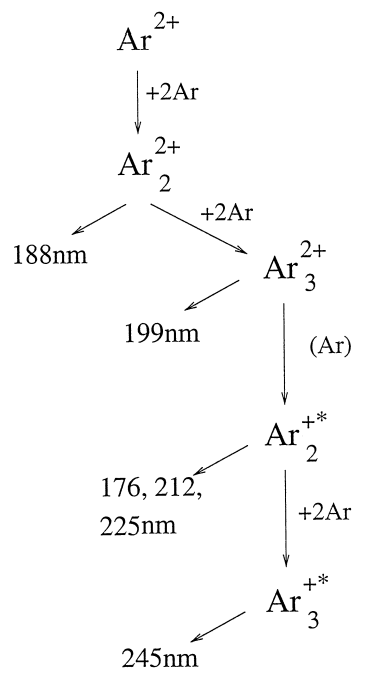
\includegraphics[width=0.8\linewidth]{experimental_espectra/3erContinuo.png} 
    \captionof{figure}{$\Ar_{\third}$ decaimientos \cite{WIESER2000233}.}   
    \label{fig:3erContinuo}
\end{minipage}

\vspace*{1em}

\begin{figure}[htbp]
    \centering
    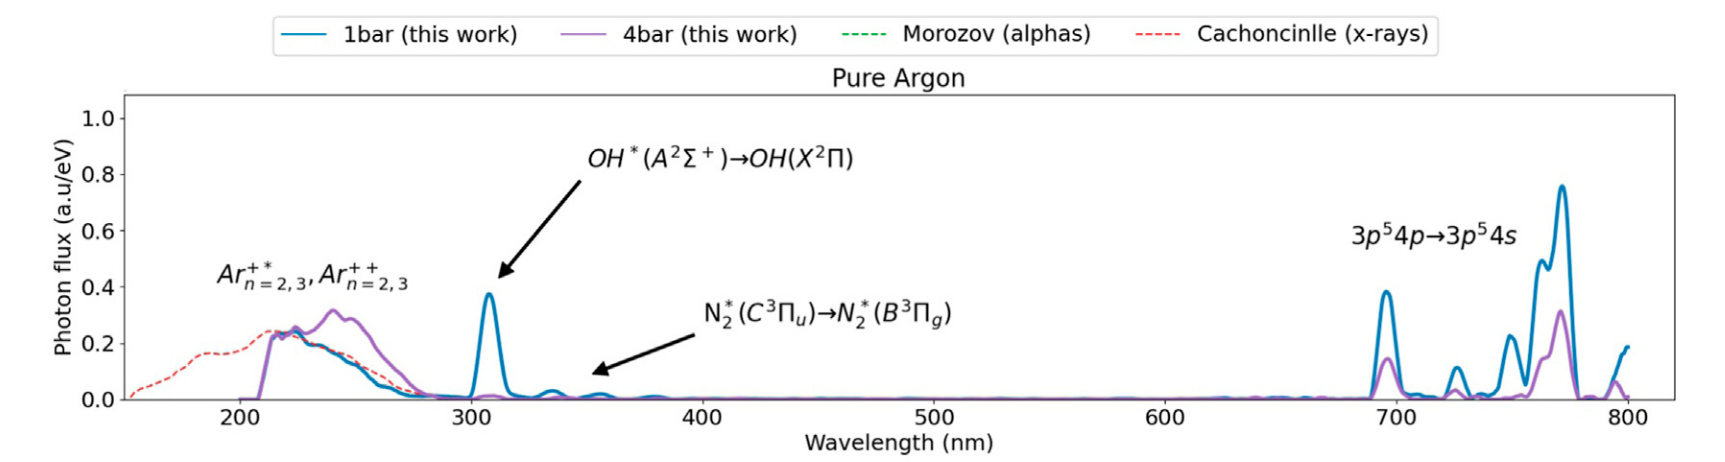
\includegraphics[width=\linewidth]{experimental_espectra/ArEspectroCompleto.png}
    \caption{Espectro experimental 200-800 nm por rayo X en argón puro \cite{amedo2023observation}.}
    \label{fig:experimentalArGlobalEspectra}
\end{figure} 

Como ya hemos dicho, en la región del infrarrojo cercano (NIR), el argón emite varias líneas atómicas asociadas a transiciones \(3p^5 4p \rightarrow 3p^5 4s\), descritas en la notación de Paschen como \(2p_n \rightarrow 1s_m\). En nuestro rango de estudio será especialmente relevante las transiciones de la tabla \ref{tab:ArNIRlines}. 

\begin{table}[htbp]
    \centering
    \caption{Principales líneas NIR del argón consideradas en este trabajo \cite{Wiese1989Argon}.}
    \label{tab:ArNIRlines}
    \begin{tabular}{cccc}
        \toprule
        $\lambda$ (nm) & Transición & $\tau$ [ns] \\
        \midrule
        696 & $2p_2 \rightarrow 1s_5$ & 28.3 \\
        727 & $2p_2 \rightarrow 1s_4$ & 28.3 \\
        750 & $2p_1 \rightarrow 1s_2$ & 21.7 \\
        763 & $2p_6 \rightarrow 1s_5$ & 29.4 \\
        772 & $2p_2 \rightarrow 1s_3$ & 28.3 \\
        794 & $2p_4 \rightarrow 1s_3$ & 29.4 \\
        \bottomrule
    \end{tabular}
\end{table}


\subsection{CF$_4$}

En el \CFt centellea, en el rango de interés, a traves del decaimiento de dos especies, el $\CF_4^{+.*}$ y el $\CF_3^*$. La región del visible, con un pico de 630 nm, está asociada a la transición 

$$\CF_3^*(2A_2'',1E') \rightarrow \CF_3(1A_1') + h \nu (\SI{630}{nm})$$ 

\cite{washida1983emission}. En el ultravioleta tenemos varias especies que pueden centellear. Las emisiones predominantes en el primario son las asociadas a 

$$\CF_4^{+,*} (\tilde{C}) \rightarrow  \CF_4^{+,*} (\tilde{A},\tilde{X})+ h \nu (\SI{290}{},\SI{230}{nm})$$ 

con 230 y 290 nm de emisión. La emisión por parte del $\CF_3^*$ en el ultravioleta, importante para el centelleo secundario

$$\CF_3^*(1A1') \rightarrow \CF_3(1A_1') + h \nu (\SI{260}{nm})$$ 

Por otro lado, también está presente la transición 

$$\CF_4^{+,*} (\tilde{D}) \rightarrow  \CF_4^{+,*} (\tilde{A})+ h \nu (\SI{364}{nm})$$ 

En la imagen \ref{fig:experimentalCF4GlobalEspectra} podemos ver las emisiones del \CFt \ puro.

\begin{figure}[htbp]
    \centering
    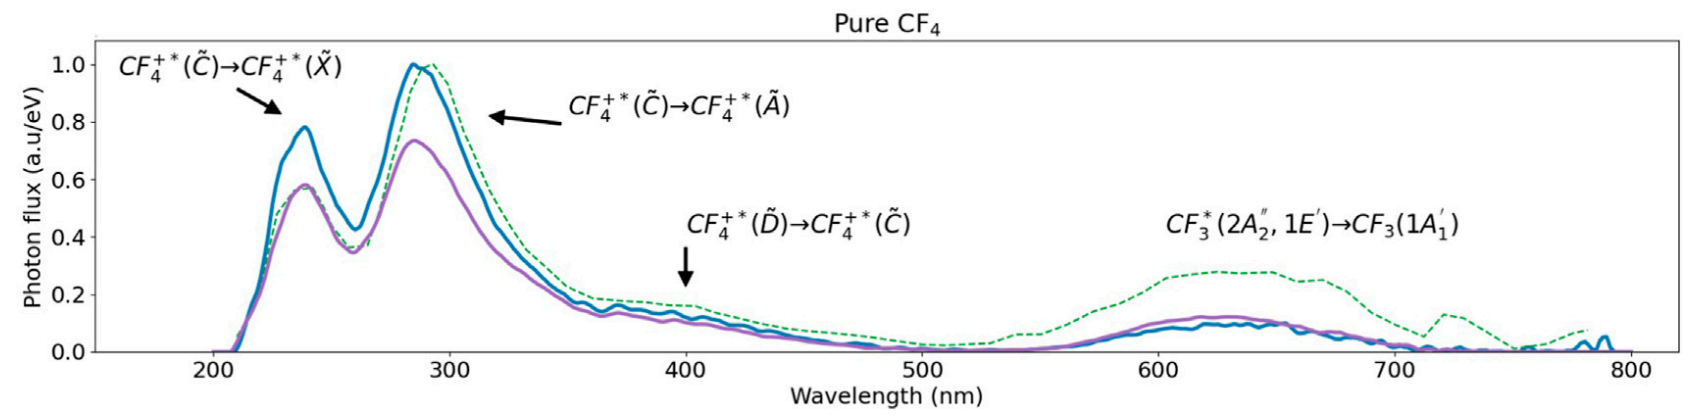
\includegraphics[width=\linewidth]{experimental_espectra/CF4EspectroCompleto.png}
    \caption{Espectro experimental 200-800 nm por rayo X en \CFt \ puro \cite{amedo2023observation} . Leyenda en la imagen \ref{fig:experimentalArGlobalEspectra}.}
    \label{fig:experimentalCF4GlobalEspectra}
\end{figure}


\subsection{Ar--CF$_4$ y He--CF$_4$}

Tras introducir las emisiones individuales del argón y del CF$_4$, se consideran las dos mezclas objeto del documento. En Ar--CF$_4$ se abren canales de transferencia energética que no existen en los gases puros. En la figura~\ref{fig:experimentalArCF4GlobalEspectra} la emisión visible del CF$_4$ aparece ya a concentraciones bajas de aditivo y puede superar la observada en CF$_4$ puro, pese a estar asociada al $\CF_3^*$. Este comportamiento es una manifestación directa del \emph{wavelength shifting}; un efecto análogo, aunque más sutil, puede contribuir también a la región ultravioleta del $\CF_4^{+,*}$.

\begin{figure}[h!]
    \centering
    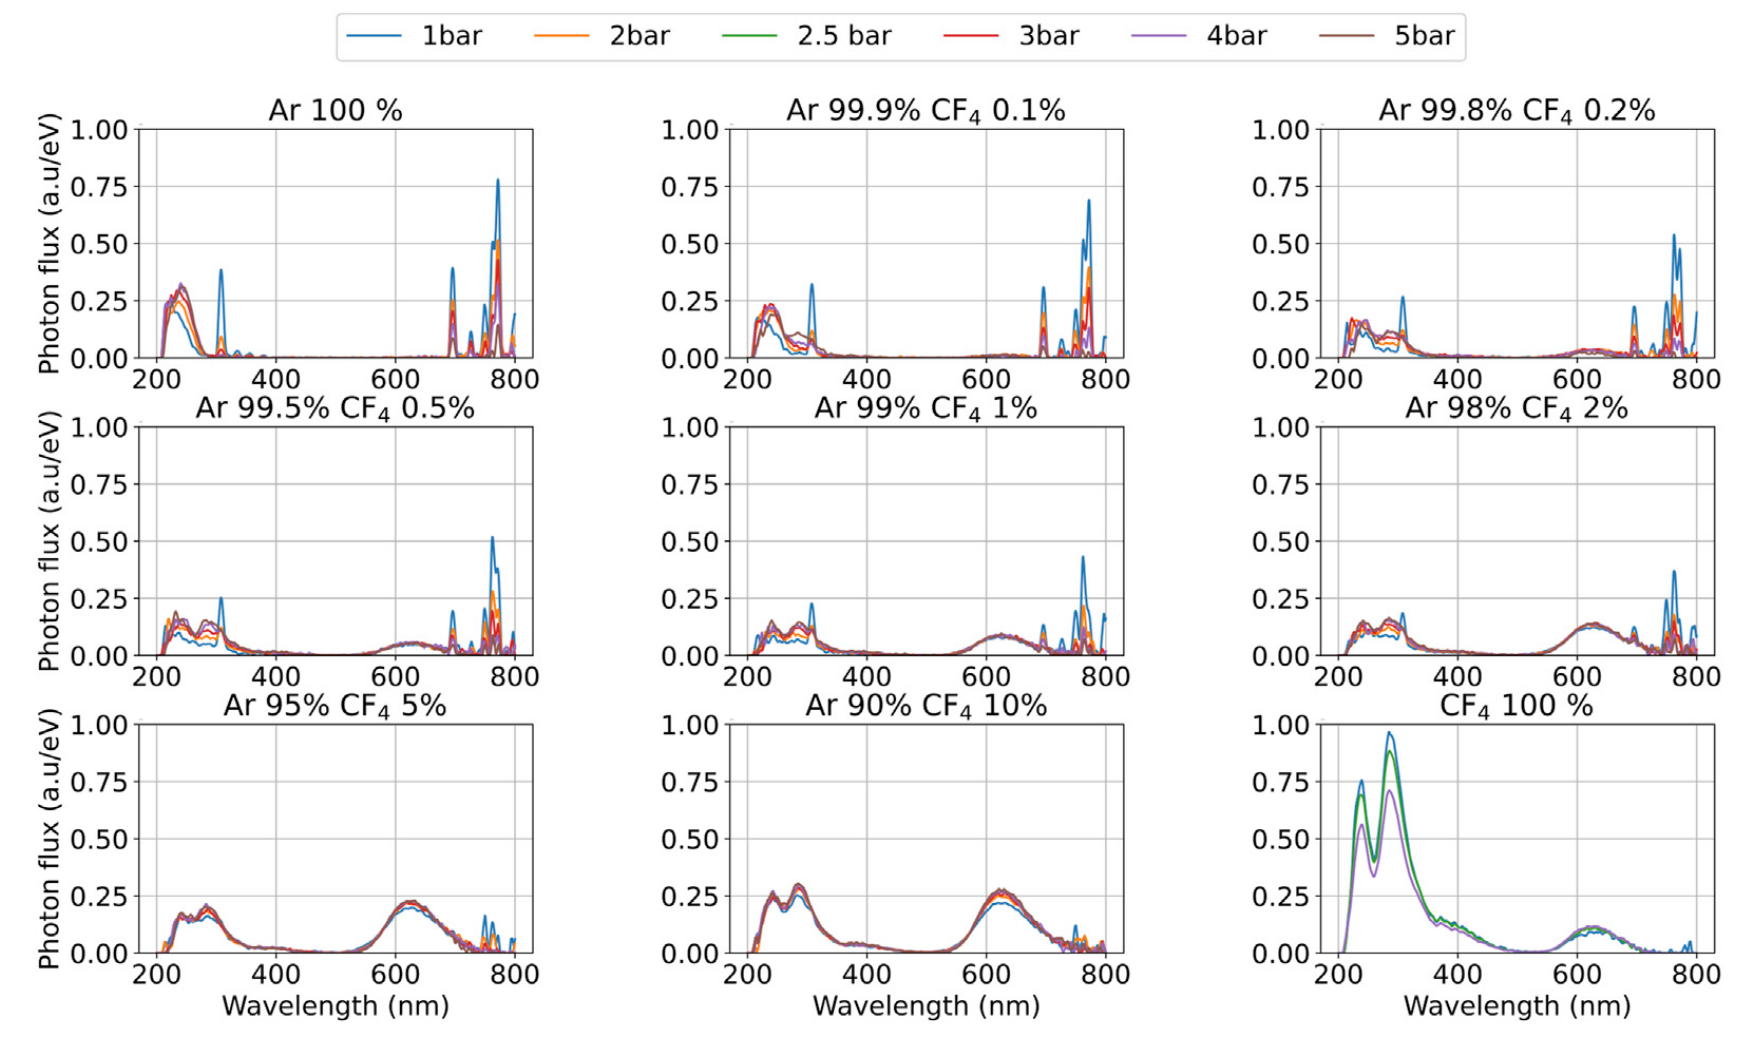
\includegraphics[width=0.95\linewidth]{experimental_espectra/ArCF4-Abosuluto.png}
    \caption{Espectro experimental absoluto de la mezcla Ar--CF$_4$ \cite{amedo2023observation}.}
    \label{fig:experimentalArCF4GlobalEspectra}
\end{figure}

El caso de He--CF$_4$ es diferente: al no esperarse una transferencia energética comparable en el rango 200--800 nm, su centelleo se interpreta como producción directa de las especies emisoras del CF$_4$. El helio funciona así como gas base de control para comprobar los parámetros directos usados en el modelo de Ar--CF$_4$.

\begin{minipage}{0.48\linewidth}
    \centering
    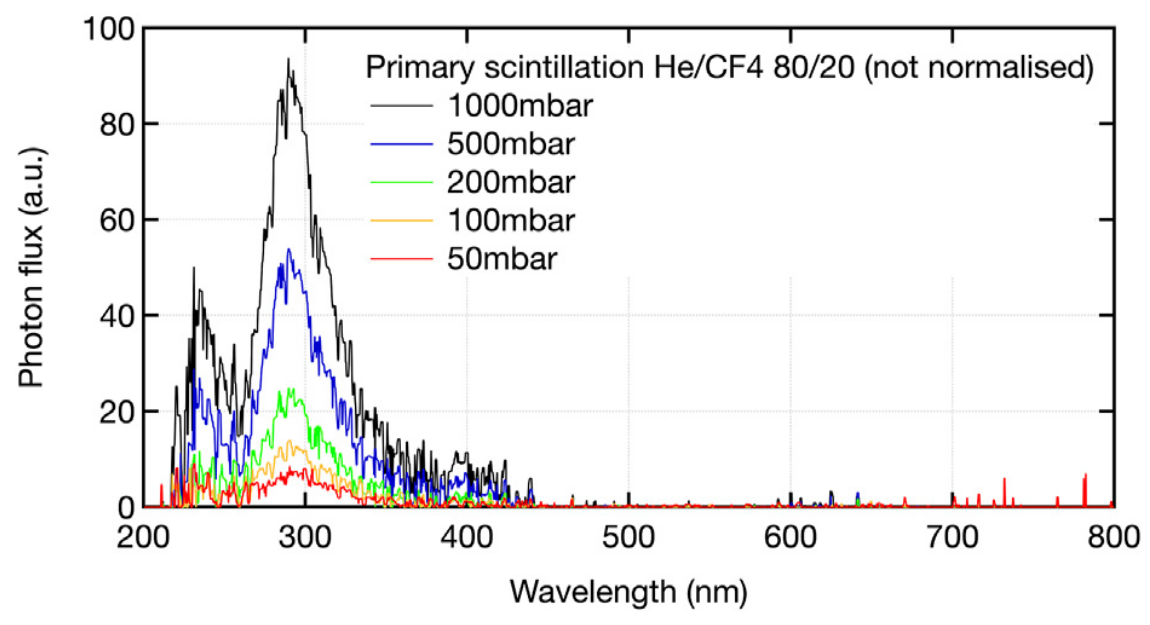
\includegraphics[width=0.9\linewidth]{experimental_espectra/HeCF4_primary.png}
    \captionof{figure}{Centelleo primario de He--CF$_4$ con partículas $\alpha$; predominan los picos ultravioletas del $\CF_4^{+,*}$ \cite{FlorianPrimarySecundary}.}
    \label{fig:HePrimary}
\end{minipage} \hfill
\begin{minipage}{0.48\linewidth}
    \centering
    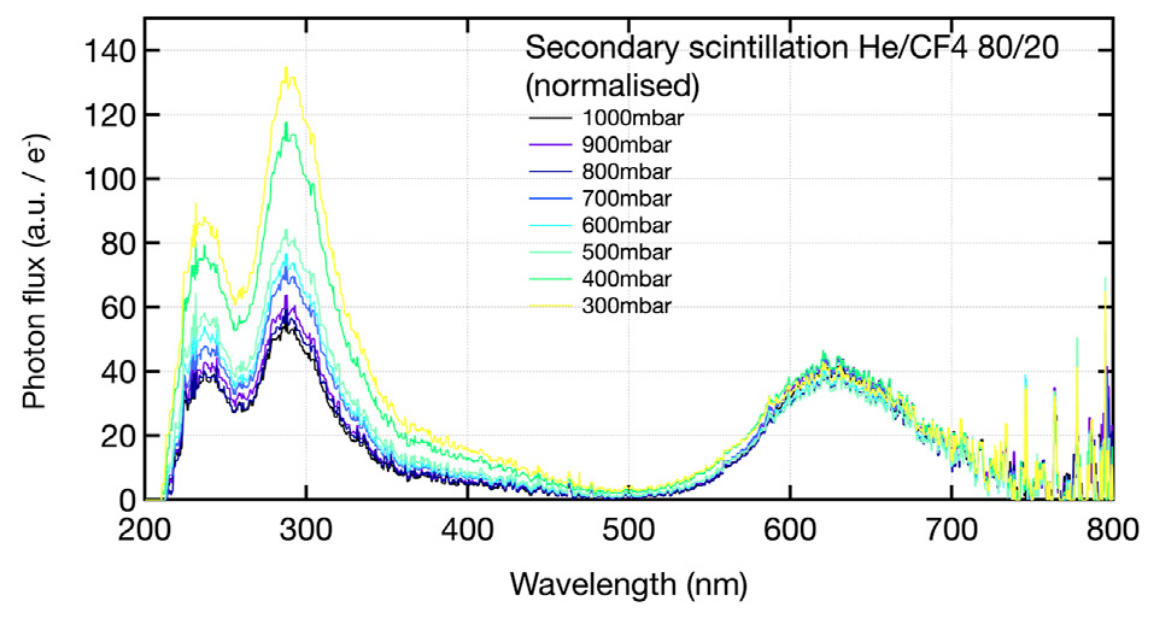
\includegraphics[width=0.99\linewidth]{experimental_espectra/HeCF4_sec.png}
    \captionof{figure}{Centelleo secundario de He--CF$_4$ en TH-GEM, con contribuciones visible y ultravioleta \cite{FlorianPrimarySecundary}.}
    \label{fig:HeSec}
\end{minipage}

\section{Modelo Cinético} \label{Sec:model_kin}
% =================================================

\subsection{Introducción a los modelos cinéticos}


Los modelos cinéticos para la descripción de gases son herramientas análogas a los modelos radiativo-colisionales de la física de plasmas. Su objetivo es describir la evolución de las poblaciones de átomos, moléculas, iones y estados excitados cuando actúan simultáneamente procesos de producción, transferencia de energía, relajación colisional y emisión radiativa. En muchos problemas de centelleo no es necesario seguir la función de distribución completa de las partículas, sino que basta con describir la dinámica de las poblaciones de las especies relevantes mediante ecuaciones de balance.

Para una especie o estado excitado \(i\), la ecuación cinética general puede escribirse como
\begin{equation}
    \dv{N_i}{t}
    =
    S_i
    +
    \sum_j N_j R_{j\to i}
    -
    N_i \sum_k R_{i\to k},
    \label{eq:general_kinetic_balance}
\end{equation}
donde \(N_i\) es la población de la especie \(i\), \(S_i\) representa su producción directa, y los coeficientes \(R_{j\to i}\) y \(R_{i\to k}\) agrupan las tasas de formación y destrucción debidas a colisiones, transferencias de carga, disociaciones, relajaciones no radiativas o decaimientos radiativos.

En el caso de un estado excitado concreto, la destrucción suele venir dada por la competencia entre emisión espontánea y desexcitación colisional. Si el estado \(i\) posee una vida media radiativa \(\tau_i\) y puede ser desactivado por colisión con distintas especies \(m\), de densidad \(n_m\), con coeficientes cinéticos \(K_{iQ(m)}\), entonces la tasa total de desaparición del estado viene dada por
\begin{equation}
    \Gamma_i^{\text{tot}}
    =
    \frac{1}{\tau_i}
    +
    \sum_m n_m K_{iQ(m)}.
    \label{eq:total_loss_rate}
\end{equation}

Bajo condiciones estacionarias, \(\dv*{N_i}{t}=0\), la población del estado queda determinada por el cociente entre su tasa total de producción y su tasa total de pérdida:
\begin{equation}
    N_i
    =
    \frac{S_i + \sum_j N_j R_{j\to i}}
    {\Gamma_i^{\text{tot}}}.
    \label{eq:stationary_population}
\end{equation}

Más útil que la población absoluta es, en muchos casos, la probabilidad de que un estado excitado evolucione a través de un canal concreto. Si un proceso \(x\) compite con el resto de canales de desexcitación, su probabilidad viene dada por la razón entre su tasa parcial y la tasa total:
\begin{equation}
    P_{i\to x}
    =
    \frac{\Gamma_{i\to x}}
    {\Gamma_i^{\text{tot}}}.
    \label{eq:branching_ratio_general}
\end{equation}
De este modo, si el canal \(x\) corresponde a una colisión con una especie \(m\), se obtiene
\begin{equation}
    P_{i\to m}
    =
    \frac{n_m K_{iQ(m)}}
    {\dfrac{1}{\tau_i} + \sum_\ell n_\ell K_{iQ(\ell)}},
    \label{eq:branching_collision}
\end{equation}
mientras que si el canal considerado es radiativo,
\begin{equation}
    P_{i\to \gamma}
    =
    \frac{1/\tau_i}
    {\dfrac{1}{\tau_i} + \sum_\ell n_\ell K_{iQ(\ell)}}.
    \label{eq:branching_radiative}
\end{equation}

En una mezcla binaria genérica \(A-B\), con densidad total \(n\) y fracción molar \(f\) de \(A\), las densidades parciales vienen dadas por
\begin{equation}
    n_{A}=n\,f,
    \qquad
    n_{B}=n\,(1-f).
\end{equation}
Por tanto, las probabilidades de evolución de un estado excitado quedan fijadas por la competencia entre los canales de colisión con argón, los canales de colisión con el aditivo molecular y los decaimientos radiativos intrínsecos. Esta estructura conduce directamente a expresiones del tipo
\begin{equation}
    P
    =
    \frac{n\,f\,K_{\text{canal}}}
    {n\,f\,K_{\text{canal}}
    +
    n\,(1-f)\,K_{\text{competencia}}
    +
    1/\tau},
    \label{eq:generic_probability_binary_mixture}
\end{equation}
que son precisamente las que aparecen en el modelo cinético empleado para describir el centelleo en $\Ar-\CF_4$ y, al suprimir los canales de transferencia desde el argón, en $\He-\CF_4$. La constante de Loschmidt 

$$ n_0 = \SI{2.6868e25}{m^{-3}} $$

nos da el número de moléculas que hay en un gas ideal a 1 atm y a 273.15 K. Así pues, si solo modificamos la presión siempre podemos expresar la densidad molar como:  

$$ n = (p/p_0) \cdot  n_0 $$

Nosotros incluiremos esta $n_0$ dentro de los coeficientes cinéticos $K$, que ahora tendrán unidades de ns$^{-1}$. Denotaremos a partir de ahora $n=p/p_0$ siendo $p_0 = \SI{1}{bar}$.

A partir de estas probabilidades de rama, el rendimiento de emisión asociado a una determinada banda espectral puede construirse como la suma de todas las vías de producción que alimentan la especie centelleadora, ponderadas por la probabilidad de que dicha especie se forme y, posteriormente, emita radiativamente antes de ser extinguida por colisión. 

\subsection{Ar--CF$_4$} \label{subbsec:kinArCF4}

\subsubsection{Interacciones}

Para la emsión del $\CF_4(\tilde{C})^{+,*}$ y del tecer continuo, los mecanimsmos de interacción son:  

\begin{itemize}
    \item  Trasferencias y quenching del tercer continuo con $\CF_4$
    \begin{equation}
        \Ar_{n=2,3}^{+,*},
        \Ar_{n=2,3}^{++,(*)} + \CF_4
        \xrightarrow{K_{\Ar_\third Q(\CF_4)}}  2(3) \Ar^{(+)} + \CF_4^{(+,*)}
    \end{equation}
    % tal que el coeficiente cinético de que se produzca $\CF_4^{+,*}(\tilde{C},v)$ será $P_{\Ar^{++}}K_{\Ar_\third Q(\CF_4)}$
    % \begin{equation}
    %     \Ar_{n=2,3}^{+,*},
    %     \Ar_{n=2,3}^{++,(*)} + \CF_4
    %     \xrightarrow{P_{\Ar^{++}}K_{Ar_\third Q(\CF_4)}} 2(3) \Ar^{(+)} + \CF_4^{+,*}(\tilde{C},v)
    % \end{equation}
    \item Emisión del tercer continuo
    \begin{equation}
        \Ar_{n=2,3}^{+,*},
        \Ar_{n=2,3}^{++,(*)} + \CF_4
        \xrightarrow{\tau_\third} 2(3) Ar + h \nu (80-\SI{300}{nm})
    \end{equation}
    \item Relajación del $\CF_4^{+,*}(\tilde{C},v)$ a  $\CF_4^{+,*}(\tilde{C},v=0)$
    \begin{equation}
         \CF_4^{+,*}(\tilde{C},v) \xrightarrow{K_{\mathrm{relax}}}  \CF_4^{+,*}(\tilde{C},v=0)
    \end{equation}
    \item Disociación del $\CF_4^{+,*}(\tilde{C},v)$ 
    \begin{equation}
         \CF_4^{+,*}(\tilde{C},v) \xrightarrow{\tau_{\mathrm{diss}}} \text{Estados no radiativos}
    \end{equation}
    \item Emisión del $\CF_4^{+,*}(\tilde{C},v=0)$ 
    \begin{equation}
         \CF_4^{+,*}(\tilde{C},v=0) \xrightarrow{\tau_{\mathrm{uv}}}  
         \CF_4^{+,*}(\tilde{A},\tilde{X}) + h \nu (290,230\mathrm{nm})
    \end{equation}
    \item Quenching del $\CF_4^{+,*}(\tilde{C},v=0)$ con otro $\CF_4$
    \begin{equation}
         \CF_4^{+,*}(\tilde{C},v) + \CF_4 \xrightarrow{K_{\CF_4 Q(\CF_4)}} \text{Estados no radiativos}
    \end{equation}
\end{itemize}

Mientras que para la emsión del $\CF_3^*(2A2',1E1')$ tenemos que considerar: 

\begin{itemize}
    \item Quenching de estados excitados del argón $\Ar^{**}$ con argón
    \begin{equation}
         \Ar^{**} + \Ar \xrightarrow{K_{\Ar^{**},Q(\Ar)}}  \text{Estados no radiativos}
    \end{equation}
    \item Quenching del $\Ar^{**}$ con $\CF_4$
    \begin{equation}
         \Ar^{**} + \CF_4 \xrightarrow{K_{\Ar^{**},Q(\CF_4)}}  \Ar^{(*)} + \CF_3^{(*)} + \mathrm{F}^{(*)}
    \end{equation}
\end{itemize}

En la tabla \ref{tab:ArCF4litearture} podemos ver algunos de estos parámetros conocidos en la literatura mientras que en la imagen  \ref{fig:ArCF4_kinetic_model} podemos ver el conjunto de procesos presentes en la mezcla. 

\hspace*{1em}\begin{table}[h!]
    \centering
    \begin{tabular}{lcccccc}
        \toprule
        {\bf Parameter} & \cite{santorelli2021spectroscopic}  \\
        
        \midrule
        
        $1/\tau_{3rd}$ [$\unit{s^{-1}}$]  & $\SI{5.02e7}{}$  \\
        
        
        \bottomrule
    
    \end{tabular}
    \caption{Parameters in the literature}
    \label{tab:ArCF4litearture}
\end{table}

\begin{figure}[h!]
    \centering
    
\includegraphics[width=0.95\linewidth]{kinetic_models/Kinetics_Models-3.pdf}
    \caption{Esquema del modelo cinético para Ar--CF$_4$.}
    \label{fig:ArCF4_kinetic_model}
\end{figure}


\subsubsection{Modelo cinético Ar--CF$_4$}

Conociendo entones el número de precursores ($\Ar^{**},\Ar^{+,*}_{n=2,3},\Ar^{++,(*)}_{n=2,3},\CF_3^*,\CF_4^{+,*}$) que se produzcan en la interacción del rayo X o electrón podemos usar los parámetros cinéticos anteriores junto con probabilidades/fracciones efectivas para obtener el número de fotones. Las probabilidades/fracciones efectivas son necesarias porque no en algunos casos no tenemos acesso al \textit{número de estados de cada especie particular}, véase, $\CF_3^*(\tilde{C})$, si no que tendremos el \textit{número de estados generales}, véase, el número de excitaciones totales de $\CF_3^*$. Las probabilidades efectivas es un mecanismo teórico que mantiene la sencillez del modelo mientras hacemos hipótesis realistas de las trasferencias.

En el caso del ${\CF_4^{+,*}}$ usaremos $N_{\CF_3^{+}}$ en vez de $N_{\CF_4^{+,(*)}}$, ya que no tenemos disponible información acerca de estos estados. La aproximación es válida ya que el 100\% de estados del $\CF_4^{+}$ acaban disociándose en $\CF_3^{+,(*)}$ \cite{zhang1989excitation}. 

Así pues, el centelleo de una mezcla de $\Ar-\CF_4$ tiene tres componentes de emisión. La emisión del visible, por parte de la especie $\CF_3^*$, viene dada por
\begin{equation}
    Y_{\CF_3,\vis}
    =
    N_{\CF_3}\cdot \left. P_{\CF_3^*}\right|_{\vis,\dir}
    +
    N_{\Ar^{**}} \cdot P_{\Ar^{**}}
    \cdot
    \frac{n \cdot f \cdot K_{\Ar^{**}Q(\CF_4)}}{
    n \cdot f \cdot K_{\Ar^{**}Q(\CF_4)}
    +
    n \cdot (1-f) \cdot K_{\Ar^{**}Q(\Ar)}
    +
    1/\tau_{\Ar^{**}}} \label{eq:YvisCF3}
\end{equation} 
El parámetro $\left. P_{\CF_3^*}\right|_{\dir}$ será la probabilidad de que las excitaciones del $\CF_3$ ($N_{\CF_3}$) pertenezcan y que eventualmente centellee. El parámetro $P_{\Ar^{**}}$ será el producto de la fracción de estados excitados energéticamente capaces de realmente de transferir al $\CF_3^*$ y la probabilidad de que la transferencia se haga a un $\CF_3$ emisor.

La emisión del ultravioleta por la especie $\CF_4^{+,*}$ se modela como
\begin{equation}
    Y_{\CF_4,\uv}
    =
    P_{\CF_4^{+,*}}
    \cdot
    \bqty{
      N_{\CF_3^+}\cdot \left. P_{\CF_4^{+,*}} \right|_{\dir}
      +
      N_{\Ar^{++}}\cdot P_{\Ar^{++}}
      \pqty{
        \frac{n \cdot f \cdot K_{\Ar^{++}Q(\CF_4)}}{
        1/\tau_{\third} + n \cdot f \cdot K_{\Ar^{++}Q(\CF_4)}}
      }
    }. \label{eq:YuvCF4}
\end{equation} 
\begin{equation}
    P_{\CF_4^{+,*}}
    =
    \frac{n \cdot f \cdot K_{\text{relax}}}{
    n \cdot f \cdot K_{\text{relax}} + 1/\tau_{\text{dissc}}}
    \cdot
    \frac{1/\tau_{\uv}}{
    1/\tau_{\uv} + n \cdot f \cdot K_{\CF_4^{+,*}Q(\CF_4)}}.
\end{equation} 

donde $\left. P_{\CF_4^{+,*}} \right|_{\dir}$ será la fracción de estados asociados y $P_{\Ar^{++}}$ la probabilidad de interacción de un precursor del tercer continuo con un $\CF_4$ genere un $\CF_4(\tilde{C},v)$. Además también existirá la posibilidad de que el $\CF_3^*$ decaiga en 260 nm, que dado que sigue los mismos mecanismos del visible, y observacionalmente se ve que el pico es mucho menor que los del visible, podemos regular directamente como el producto de una probabilidad efectiva y la emisión en el visible, tal que
\begin{equation}
    Y_{\CF_3,\uv}
    = \left. P_{\CF_3^*}\right|_{\uv,\dir} \cdot 
    Y_{\CF_3,\vis}     \label{eq:YuvCF3}
\end{equation} 

Finalmente, la emisión ultravioleta asociada a la componente $\Ar_{\third}$ es
\begin{equation}
    Y_{\Ar_{\third},\uv}
    =
    N_{\Ar^{++}}
    \cdot
    \pqty{
      \frac{1/\tau_{\third}}{
      1/\tau_{\third} + n \cdot f \cdot K_{\Ar^{++}Q(\CF_4)}}
    }. \label{eq:YuvAr3rd}
\end{equation}

\subsection{He--CF$_4$} \label{subbsec:kinHeCF4}

Como ya hemos dicho, la mezcla He-CF$_4$ no posee fenómenos de \textit{wavelengh shifting}, de tal modo que solo haya centelleo directo, tal y como podemos ver en la imagen \ref{fig:HeCF4_kinetic_model}.


\begin{figure}[h!]
    \centering
    
\includegraphics[width=0.95\linewidth]{kinetic_models/Kinetics_Models-5.pdf}
    \caption{Esquema del modelo cinético para He--CF$_4$.}
    \label{fig:HeCF4_kinetic_model}
\end{figure}


Y por tanto las ecuaciones

\begin{equation}
    Y_{\CF_3,\vis}
    =
    N_{\CF_3}\cdot \left. P_{\CF_3^*}\right|_{\dir} \label{eq:YvisHeCF3}
\end{equation} 

\begin{equation}
    Y_{\CF_4,\uv}
    = \pqty{
    \frac{n \cdot f \cdot K_{\text{relax}}}{
    n \cdot f \cdot K_{\text{relax}} + 1/\tau_{\text{dissc}}}
    \cdot
    \frac{1/\tau_{\uv}}{
    1/\tau_{\uv} + n \cdot f \cdot K_{\CF_4^{+,*}Q(\CF_4)}}
    \cdot}
    \pqty{
      N_{\CF_3^+}\cdot \left. P_{\CF_4^{+,*}} \right|_{\dir}
      }
      \label{eq:YuvHeCF4}
\end{equation} 

\begin{equation}
    Y_{\CF_3,\uv}
    = \left. P_{\CF_3^*}\right|_{\uv,\dir} \cdot 
    Y_{\CF_3,\vis}    
     \label{eq:YuvHeCF3}
\end{equation}

que como podemos ver son iguales a las de los de las ecuaciones \ref{eq:YvisCF3}, \ref{eq:YuvCF4} y \ref{eq:YuvCF3} si eliminamos las transferencias del Argón. 

\subsection{Infrarrojo en Ar--CF$_4$} \label{subbsec:kinArIR}

Los mecanismos de interacción que consideraremos son. 

\begin{minipage}{0.55\linewidth} 
\begin{itemize}
    \item Decaimiento de la especie: 
    
    \begin{equation}
        \Ar^*_\lambda \xrightarrow{\tau_{\Ar^*_\lambda}}  \Ar + h\nu (\lambda 
  \ \mathrm{nm})
    \end{equation}
    
    \item Quenching con argón:

    \begin{equation}
        \Ar^*_\lambda +  \Ar
        \xrightarrow{K_{\Ar^*_\lambda,Q(\Ar)}}  \text{Estados no radiativos}
    \end{equation}
    
    \item Quenching con un aditivo molecular $(\CF_4)$: 

    \begin{equation}
        \Ar^*_\lambda + X       \xrightarrow{K_{\Ar^*_\lambda,Q(\CF_4)}}  \text{Estados no radiativos}
    \end{equation}
    
\end{itemize}
\end{minipage} \hfill
\begin{minipage}{0.42\linewidth} \centering
    
\includegraphics[width=0.96\linewidth]{kinetic_models/Kinetics_Models-4.pdf}
    \captionof{figure}{Modelo cinético Ar IR.} \label{fig:Ar_IR_kinetic_model}
\end{minipage}


Las emisiones del infrarrojo del Ar se producen por especies muy concretas (apartado \ref{subsec:Ar_spectra}). Estas especies no pueden producirse por mecanismos de trasferencia por parte de otras especies de argón o del aditivo molecular, por lo que solo debemos considerar la producción directa de los mismos. No obstante, si pueden producirse por el decaimiento de excitaciones más energéticas. Entonces $ N_{\Ar^*,\lambda}$ será la suma todos las excitaciones más energéticas que la que emite, y $P_{\Ar^*,\lambda}$ será el producto de la fracción de estados realmente involucrados y la probabilidad de que estos lleven a la especie centelladora. Una vez llegan a esta entra la competencia entre decaimiento y fenómenos de quenching (véase figura \ref{fig:Ar_IR_kinetic_model}). Así el modelo cinético de la emisión infrarroja para el pico de longitud de onda $\lambda$

\begin{equation}
    Y_{\mathrm{IR},\lambda} = P_{\Ar^*,\lambda} \cdot N_{\Ar^*,\lambda}  \cdot \pqty{\frac{1 / \tau_{\Ar^*,\lambda}}{1 / \tau_{\Ar^*,\lambda} + n \cdot f \cdot  K_{\Ar^*, Q(\Ar), \lambda} + n \cdot(1-f) \cdot  K_{\Ar^*, Q(\CF_4), \lambda}} }
\end{equation}

\section{Simulaciones} 
% =================================================

Para obtener la población media de cada estado por evento, \(N_X\), se han utilizado dos herramientas complementarias: Degrad para la descripción de la interacción primaria, y Garfield++ la descripción del centelleo secundario. Esta combinación permite separar de forma natural dos escalas físicas distintas. Por un lado, la creación del primario depende del tipo de partícula incidente y de sus mecanismos de ionización inicial. Por otro, el desarrollo de la avalancha, la producción de excitaciones y la creación de electrones secundarios están dominados por el campo eléctrico local y por las secciones eficaces electrón--átomo/molécula de la mezcla. 

Desde el punto de vista cinético, la magnitud de entrada fundamental son las secciones eficaces \(\sigma_j(\varepsilon)\) asociadas a cada canal microscópico \(j\) (colisión elástica, excitación, ionización, attachment, \emph{etc.}), donde \(\varepsilon\) es la energía cinética del electrón. En términos prácticos, esto implica que las poblaciones \(N_X\) por evento pueden interpretarse como el resultado acumulado de todas las colisiones de excitación, ionización o attachment sufridas por el electrón primario y por todos sus descendientes a lo largo de la avalancha.


Dado que en ambos casos se utiliza un conjunto consistente de secciones eficaces, las poblaciones obtenidas con Degrad y Garfield++ son comparables aunque correspondan a fenómenos distintos. En las figuras~\ref{fig:ArCs} y \ref{fig:CF4Cs} se muestran las secciones eficaces empleadas para $\Ar$ y $\CF_4$, distinguiendo canales elásticos, de ionización, \emph{attachment} e inelásticos/excitadores.

\begin{minipage}{0.5\linewidth}
    \centering
    
\includegraphics[width=0.99\linewidth]{cross_sections/Ar_cs.pdf}
    \captionof{figure}{Secciones eficaces del argón.}
    \label{fig:ArCs}
\end{minipage} \hfill
\begin{minipage}{0.5\linewidth}
    \centering
    
\includegraphics[width=0.99\linewidth]{cross_sections/CF4_cs.pdf}
    \captionof{figure}{Secciones eficaces del $\CF_4$.}
    \label{fig:CF4Cs}
\end{minipage}

\subsection{Garfield++}

{Garfield++} es un entorno en \texttt{C++} orientado a la simulación detallada de detectores gaseosos y semiconductores basados en ionización. En el contexto de gases, su interés principal reside en la posibilidad de realizar seguimiento microscópico electrón por electrón, colisión por colisión, utilizando para ello las tasas de interacción tabuladas por {Magboltz}. Dado que {Magboltz}, también desarrollado por Steve Biagi, calcula propiedades de transporte y tasas de colisión a partir de secciones eficaces microscópicas, la combinación {Garfield++} y {Magboltz} permite pasar de la microfísica de dispersión a observables macroscópicos como deriva, difusión, coeficiente de Townsend, attachment, ganancia y producción de estados excitados.

En este trabajo, Garfield++ se emplea en modo de seguimiento microscópico de los electrones. En este esquema, el electrón se propaga entre colisiones siguiendo una trayectoria clásica determinada por el campo eléctrico local. La duración del vuelo libre se muestrea a partir de la frecuencia total de colisión, y el tipo de interacción que tiene lugar al final del paso se selecciona de acuerdo con las tasas relativas de cada proceso. Este procedimiento es especialmente adecuado para mezclas con canales competitivos muy distintos entre sí, como ocurre en $\Ar$, $\He$ y $\CF_4$, donde coexisten excitación, ionización, attachment y pérdidas inelásticas con umbrales energéticos diferentes. Gaffield++ tiene la capacidad de escalar a altras energías las ele

El algoritmo utilizado por {Garfield++} para el muestreo del tiempo de vuelo es el método de Monte Carlo con colisiones nulas (\textit{null-collision Monte Carlo}, también conocido como MCC o técnica NC). La idea básica consiste en introducir una frecuencia ficticia adicional que permita muestrear los vuelos libres con una tasa mayorante simple; cuando el proceso sorteado corresponde a una ``colisión nula'', la partícula no cambia de estado físico y simplemente continúa su movimiento. Aunque estas colisiones virtuales no tienen significado físico directo, el método reproduce correctamente la estadística de los procesos reales y resulta muy eficiente cuando las tasas de colisión dependen fuertemente de la energía del electrón. De hecho, en {Garfield++} las colisiones virtuales aparecen explícitamente en la clasificación interna de procesos como \textit{virtual (null) collisions}.

\subsection{Aproximación de campo uniforme y desarrollo de la avalancha}

Para la simulación de la multiplicación secundaria se ha adoptado la geometría de deriva uniforme mostrada en la Fig.~\ref{fig:uniformDrift}. Esta aproximación consiste en suponer que, en la región efectiva donde se desarrolla la avalancha, el campo eléctrico es aproximadamente constante:
\begin{equation}
    \mathbf{E}(\mathbf{r}) \simeq E_0\, \hat{\mathbf{z}}.
\end{equation}
La hipótesis es razonable cuando el hueco de amplificación es pequeño y el objetivo principal es estimar la estadística de colisiones, la ganancia y la producción media de excitaciones, en lugar de resolver con máximo detalle las no uniformidades locales de la geometría real. Bajo esta aproximación, las diferencias entre electrones vienen dadas sobre todo por la secuencia aleatoria de colisiones, y no por variaciones geométricas del campo.

La avalancha electrónica se construye entonces de manera jerárquica. El electrón primario, introducido directamente en {Garfield++}, atraviesa la región de deriva y, si su energía entre colisiones supera los umbrales relevantes, puede producir excitaciones o ionizaciones. Cada colisión de ionización genera un nuevo electrón secundario que, a su vez, es transportado microscópicamente por el mismo algoritmo y puede originar ionizaciones adicionales. El resultado final es una cascada ramificada, tal y como podemos ver en la figura \ref{fig:uniformDrift} en la que el primario y todos sus descendientes contribuyen a la ganancia total y a las poblaciones \(N_X\) de las distintas especies excitadas. En la figura \ref{fig:gainNe} podemos ver un histograma donde vemos el número de electrones genreados por electrón primario simulado (electrón inicial). A este número se le llama ganancia electrónica (o de carga) y se la denota como $n_e$. 

Desde el punto de vista del modelo cinético, esta cascada puede resumirse como una suma sobre trayectorias electrónicas. Si \(N_X^{(k)}\) es el número de veces que el proceso \(X\) aparece en la historia del electrón \(k\), el número total por evento viene dado por
\begin{equation}
    N_X = \sum_{k \ \in \ \mathrm{avalancha}} N_X^{(k)}.
    \label{eq:NX_event}
\end{equation}
Equivalentemente, en promedio, \(N_X\) queda determinado por la integral de las probabilidades de colisión a lo largo de todas las trayectorias del primario y de los secundarios. Esta es precisamente la magnitud que después se introduce en el modelo cinético-radiativo para estimar los distintos canales de emisión de la mezcla.



\begin{minipage}{0.43\linewidth}
    \centering
    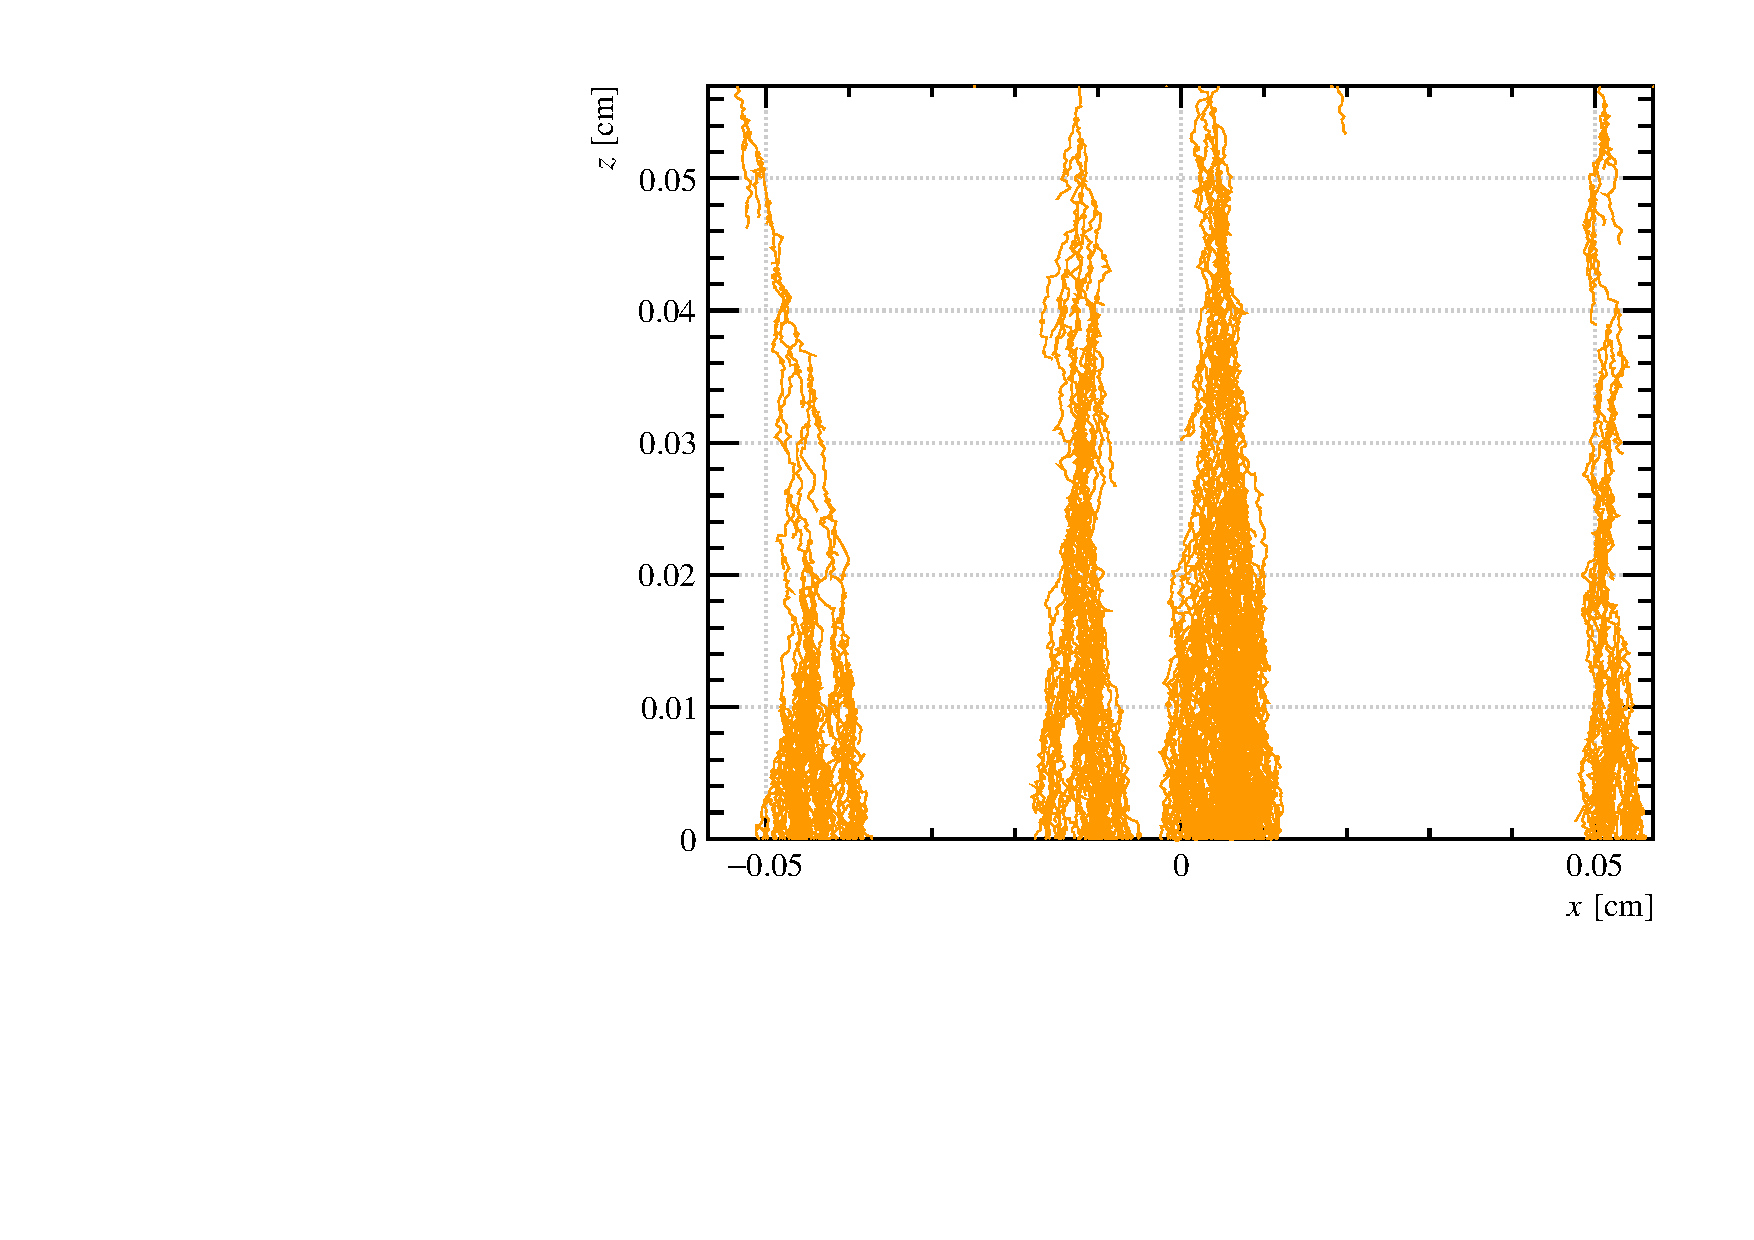
\includegraphics[width=0.99\linewidth]{garfield++/uniform_drift.pdf}
    \captionof{figure}{Cascada.}
    \label{fig:uniformDrift}
\end{minipage}
\hfill
\begin{minipage}{0.55\linewidth}
    \centering
    
\includegraphics[width=0.95\linewidth]{garfield++/cf4_100.0_ar_0.0_95.0kVcm_1.0bar_0.0500mm_1000npe_ne.pdf}
    \captionof{figure}{Distribución de ganancia electrónica simulada.}
    \label{fig:gainNe}
\end{minipage}

%\begin{minipage}{0.48\linewidth}
%    \centering
%    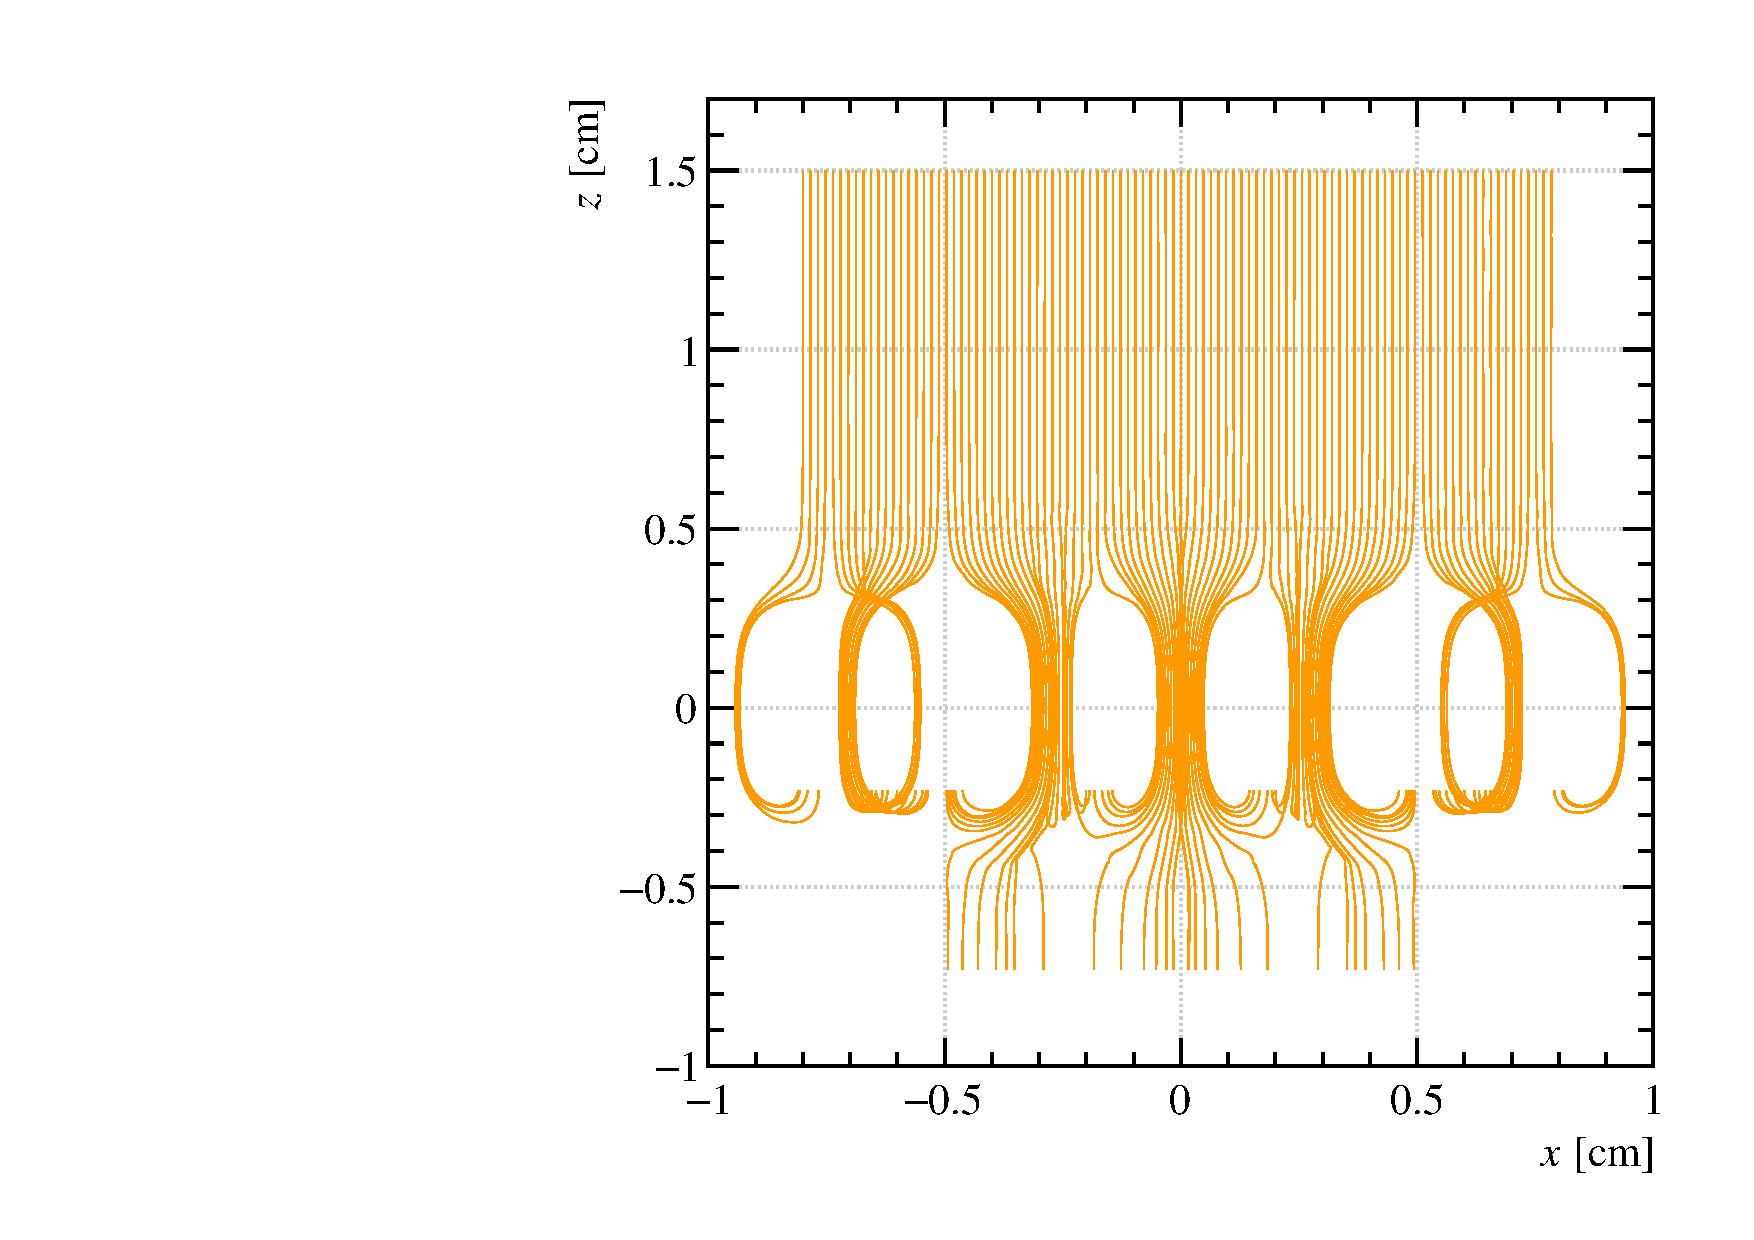
\includegraphics[width=0.99\linewidth]{garfield++/fieldLines.pdf}
%    \captionof{figure}{Líneas de campo en la estructura simulada.}
%    \label{fig:fieldLinesFatGem}
%\end{minipage}
%\hfill
%\begin{minipage}{0.48\linewidth}
%    \centering
%    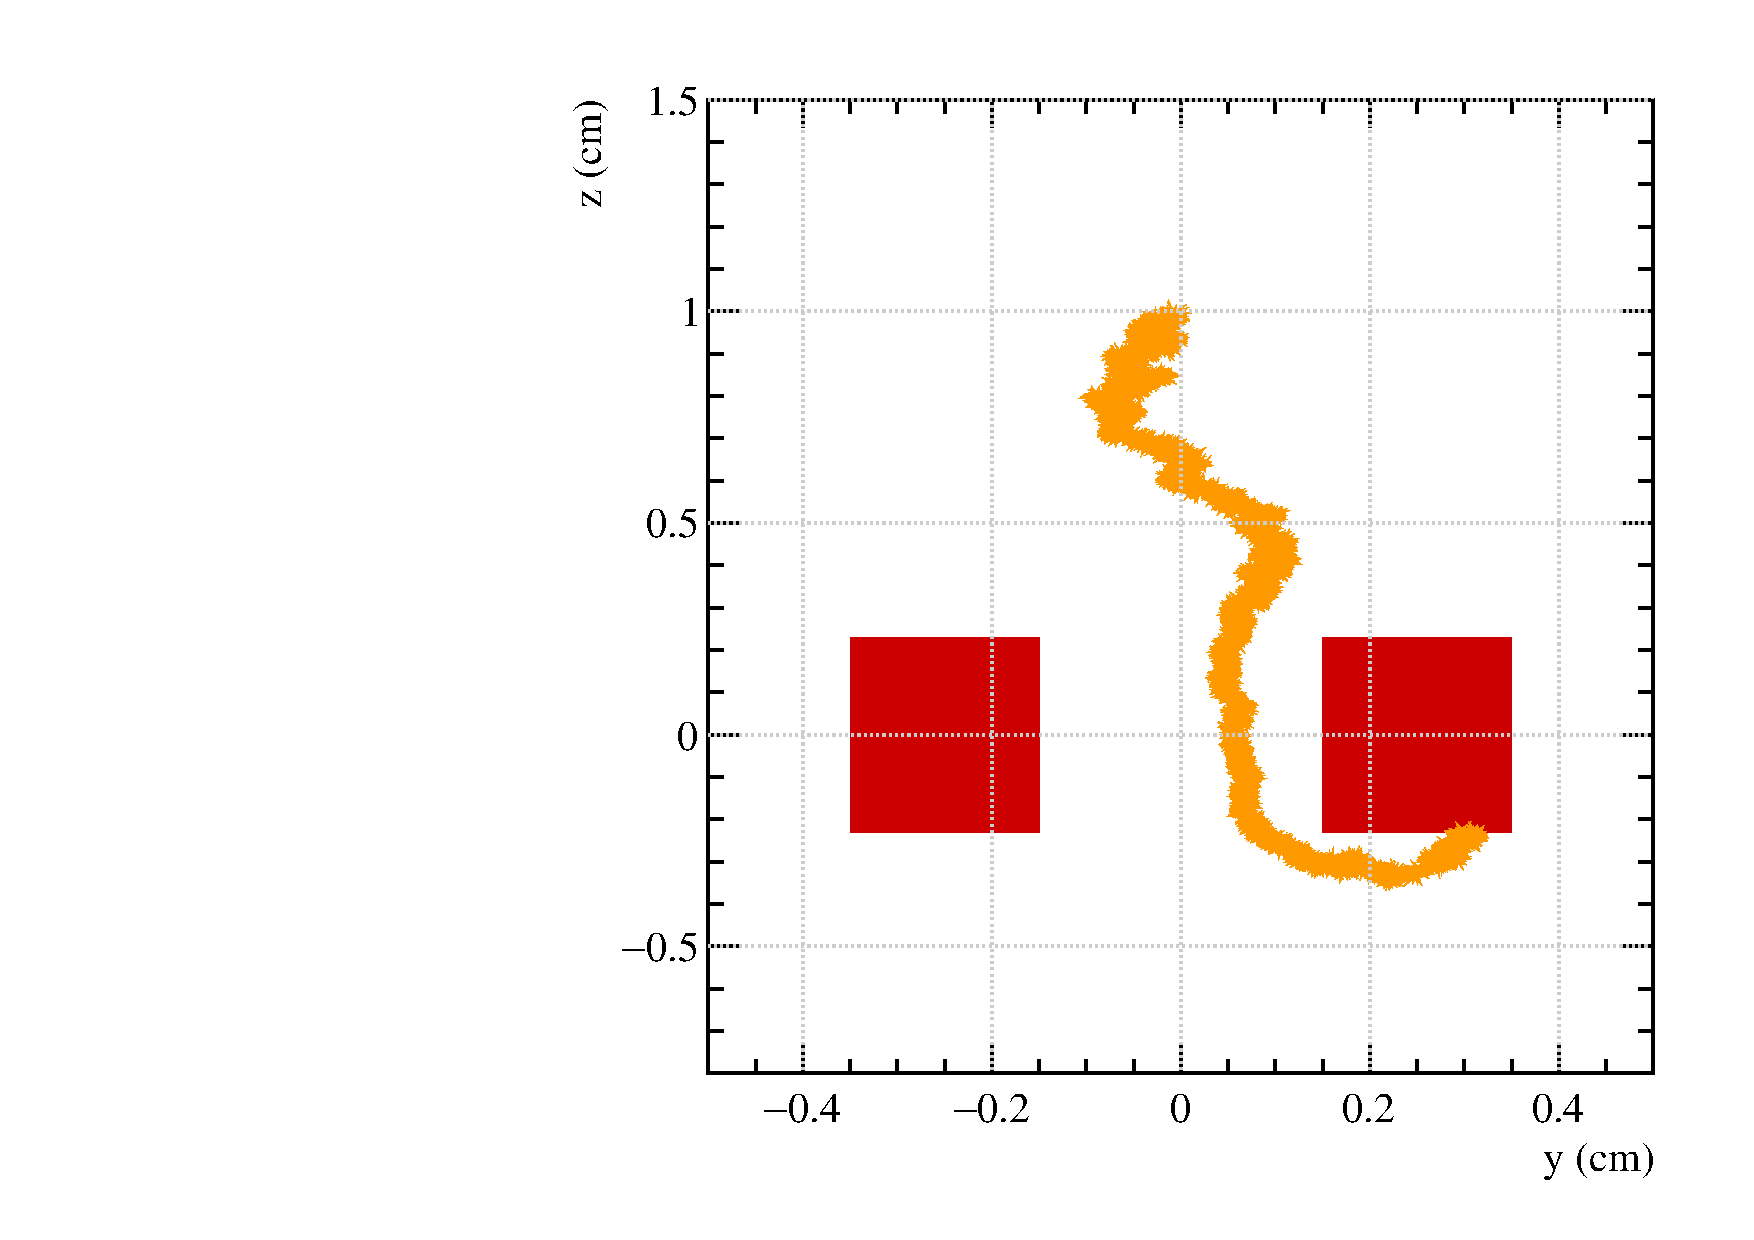
\includegraphics[width=0.99\linewidth]{garfield++/driftLine_2d.pdf}
%    \captionof{figure}{Líneas de deriva 2D en fatGem.}
%    \label{fig:driftLiensFatGem}
%\end{minipage}

% =================================================

% =================================================
\section{Obtención de Parámetros}
% =================================================

Muchos parámetros del modelo de Ar--CF$_4$ no se conocen con la precisión requerida para una predicción directa del centelleo: algunos coeficientes de \emph{quenching} y vidas medias deben determinarse a partir de los datos, mientras que ciertas probabilidades efectivas incorporan la fracción de poblaciones simuladas que alimenta realmente cada canal radiativo. Para obtenerlos se ajustan simultáneamente los rendimientos experimentales y las poblaciones calculadas con Degrad en las mismas condiciones de presión y concentración.

Los datos visibles y ultravioletas disponen de una normalización experimental común, por lo que se introduce un factor $N_{\norma}$ en las ecuaciones de rendimiento. Además, la conversión entre las poblaciones simuladas y el rendimiento observado utiliza el potencial medio de ionización $W_I(f)$ de la mezcla Ar--CF$_4$, interpolado a las concentraciones consideradas a partir de los valores experimentales disponibles \cite{reinking1986studies}. Dado que los datos cubren dos intervalos espectrales integrados, el ajuste se realiza sobre $Y_{\vis}$ y $Y_{\uv}$, sin separar experimentalmente todas las contribuciones solapadas en la región ultravioleta.

\subsection{Tratamiento de errores sistemáticos y estadísticos}

Los datos experimentales empleados en el ajuste presentan, en general, dos contribuciones principales a la incertidumbre: una componente estadística y una componente sistemática. Ambas tienen un origen físico y experimental distinto, por lo que no deben tratarse de la misma manera. Las incertidumbres estadísticas describen fluctuaciones aleatorias independientes asociadas, por ejemplo, al número finito de eventos, a la dispersión de las medidas o al proceso de extracción de los puntos experimentales. En cambio, las incertidumbres sistemáticas suelen estar asociadas a efectos comunes de calibración, eficiencia óptica, normalización, respuesta espectral o escala absoluta de intensidad. Por tanto, mientras que la componente estadística puede considerarse, en primera aproximación, independiente punto a punto, la componente sistemática debe tratarse como una fuente de desplazamiento correlacionado entre varios puntos de un mismo conjunto de datos. Esta distinción es habitual en el análisis estadístico de experimentos de física de partículas, donde las incertidumbres sistemáticas se introducen mediante parámetros auxiliares o \textit{nuisance parameters} gaussianamente constreñidos \cite{Barlow2002,Cowan2011,Conway2011,Cranmer2012HistFactory,PDGStatistics2024}.

En este trabajo, el ajuste nominal se realiza empleando las incertidumbres estadísticas de los datos experimentales. Dado un modelo $f(x;\boldsymbol{\theta})$, donde $\boldsymbol{\theta}$ representa el vector de parámetros libres, los parámetros óptimos $\hat{\boldsymbol{\theta}}$ se obtienen minimizando la suma de residuos ponderados,

\[
r_i(\boldsymbol{\theta})=
\frac{y_i-f(x_i;\boldsymbol{\theta})}
{\sigma_{i,\mathrm{stat}}},
\]

mediante la rutina \texttt{least\_squares} de \texttt{scipy.optimize} \cite{Virtanen2020SciPy}. Esta elección define la curva central del modelo, que se interpreta como la mejor descripción de los datos bajo las hipótesis físicas incorporadas al modelo. El uso exclusivo de la incertidumbre estadística en la función objetivo evita que las componentes sistemáticas, que no representan fluctuaciones independientes, sean tratadas como ruido aleatorio punto a punto. En particular, incluir directamente las incertidumbres sistemáticas en cuadratura dentro de cada residuo produciría un ajuste menos sensible a la estructura de los datos y, además, ignoraría las correlaciones entre puntos inducidas por una misma fuente sistemática.

Para propagar las incertidumbres a los parámetros y a las predicciones del modelo, se emplea un procedimiento basado en pseudoexperimentos. Este método resulta especialmente adecuado en el presente caso, ya que el modelo es no lineal y presenta degeneraciones importantes entre algunos parámetros. En estas condiciones, la estimación local de la matriz de covarianzas a partir del jacobiano del ajuste,

\[
\mathrm{Cov}(\hat{\boldsymbol{\theta}})
\simeq
s^2(J^TJ)^{-1},
\]

puede ser numéricamente inestable o difícil de interpretar. En particular, parámetros individuales pueden tener incertidumbres muy grandes debido a correlaciones internas del modelo, aunque la predicción física final permanezca relativamente bien determinada. Por este motivo, se prefiere propagar las incertidumbres directamente mediante réplicas fluctuadas de los datos y refitear el modelo en cada una de ellas. Este procedimiento es equivalente, en la práctica, a una propagación Monte Carlo de las incertidumbres experimentales y evita depender únicamente de una aproximación lineal alrededor del mínimo.

Para la componente estadística se generan pseudoexperimentos fluctuando cada punto de forma independiente,

\[
y_i^{(t)}
= 
y_i
+
\epsilon_i^{(t)},
\qquad
\epsilon_i^{(t)}
\sim
\mathcal{N}(0,\sigma_{i,\mathrm{stat}}),
\]

donde $t$ identifica la réplica generada. Cada conjunto fluctuado se ajusta de nuevo con el mismo modelo, obteniendo un vector de parámetros $\boldsymbol{\theta}^{(t)}$ y una predicción asociada $f(x;\boldsymbol{\theta}^{(t)})$. La distribución de estas predicciones proporciona una estimación directa de la incertidumbre estadística de la curva ajustada. En las figuras, la banda estadística se define mediante los percentiles 16 y 84 de las curvas obtenidas, que corresponden aproximadamente a una banda de una desviación típica para distribuciones gaussianas.

La componente sistemática se trata de forma diferente, ya que no representa fluctuaciones independientes de cada punto. Para ello se introducen variables gaussianas comunes, o \textit{nuisance parameters}, asociadas a cada fuente sistemática relevante. Si $\Delta_i^{(k)}$ representa el desplazamiento sistemático del punto $i$ debido a la fuente $k$, un pseudoexperimento sistemático se construye como

\[
y_i^{(t)}
=
y_i
+
\sum_k z_k^{(t)}\Delta_i^{(k)},
\qquad
z_k^{(t)}
\sim
\mathcal{N}(0,1).
\]

De este modo, todos los puntos afectados por una misma fuente sistemática se desplazan de forma coherente. En los datos UV y visibles de Ar--CF$_4$ se consideran fuentes sistemáticas separadas para cada región espectral, mientras que en el infrarrojo resulta natural asignar una fuente sistemática a cada longitud de onda. Este tratamiento refleja mejor el significado físico de una incertidumbre sistemática: una calibración óptica o una eficiencia espectral no desplaza cada punto al azar, sino que modifica de manera correlacionada una familia completa de medidas.

Desde el punto de vista formal, este procedimiento es equivalente a construir una matriz de covarianza total con una parte estadística diagonal y una parte sistemática correlacionada,

\[
V
=
V_{\mathrm{stat}}
+
V_{\mathrm{syst}},
\]

donde

\[
V_{\mathrm{stat},ij}
=
\sigma_{i,\mathrm{stat}}^2\delta_{ij},
\]
y
\[
V_{\mathrm{syst},ij}
=\sum_k
\Delta_i^{(k)}\Delta_j^{(k)}.
\]

Esta forma de escribir la matriz de covarianza muestra explícitamente que una fuente sistemática común genera correlaciones entre distintos puntos experimentales. El enfoque mediante pseudoexperimentos evita tener que construir e invertir explícitamente esta matriz en cada ajuste, pero conserva la interpretación física de las correlaciones sistemáticas. Es, por tanto, una versión sencilla y transparente del tratamiento mediante parámetros auxiliares usado de forma estándar en análisis de altas energías, como en los métodos de \textit{profile likelihood} e implementaciones tipo \textsc{HistFactory} \cite{Cowan2011,Cranmer2012HistFactory}.

Finalmente, las incertidumbres de los parámetros se obtienen a partir de la dispersión de los valores ajustados en los distintos pseudoexperimentos. Para cada parámetro se calculan por separado una contribución estadística, procedente de las réplicas con fluctuaciones independientes punto a punto, y una contribución sistemática, procedente de las réplicas con desplazamientos correlacionados. Las predicciones finales del modelo para rendimientos primarios en $\mathrm{ph/MeV}$ se acompañan de bandas construidas a partir de los percentiles de las curvas refiteadas. Este tratamiento permite separar de manera clara la estabilidad estadística del ajuste y la sensibilidad a fuentes sistemáticas comunes, manteniendo al mismo tiempo una interpretación física coherente de ambas contribuciones. En los casos donde algunos parámetros presentan incertidumbres relativas grandes, estas deben interpretarse con cautela, ya que pueden reflejar degeneraciones internas del modelo más que una pérdida equivalente de precisión en la predicción final. Por ello, en este trabajo se da especial importancia a las bandas de predicción del modelo, que constituyen una estimación más robusta de la incertidumbre sobre las magnitudes físicamente observables.


\subsection{Identificación de Ar$^{**}$ y CF$_3^*$}

Como ya hemos dicho, algunos de estos parámetros que hemos obtenido no se corresponden a parámetros cinéticos directamente, si no fracciones de estados de Degrad realmente involucrados. En particular $P_{\Ar^{**}}$ y $P_{\CF_3|_{\vis,\dir}}$ son parámetros que en realidad son el producto de una probabilidad (magnitud física) y una fracción (fracción de estados de Degrad relacionables con las poblaciones centelleadoras). Con el primario no tenemos capacidad de separar este producto. Para ello necesitaríamos unos datos con una distribución de poblaciones diferentes. En nuestro caso si poseemos estos datos, a saber, la información del secundario, tal y como mostramos en las imágenes \ref{fig:Arcumulative} y \ref{fig:CF3cumulative}.

\begin{minipage}{0.48\linewidth}
    \centering
    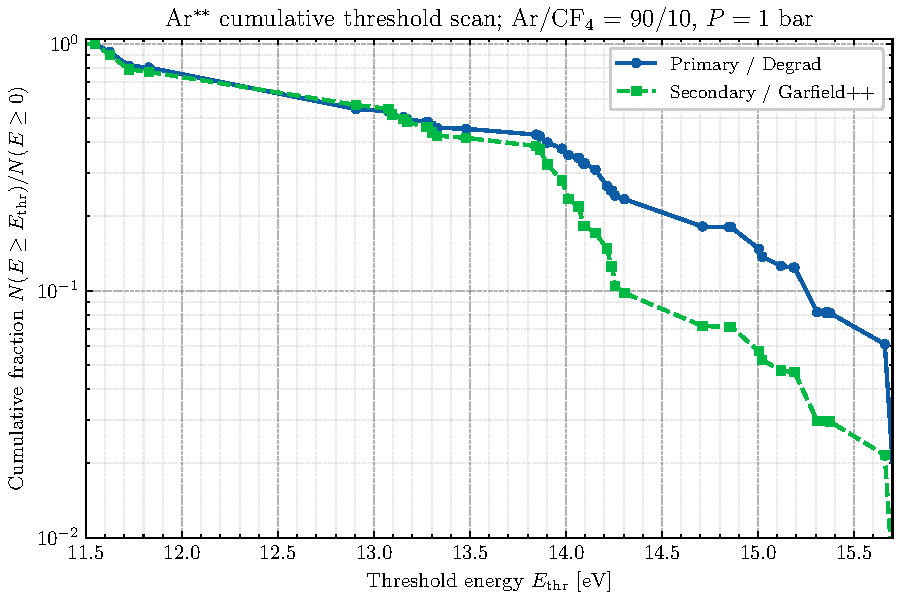
\includegraphics[width=0.99\linewidth]{cumulative/ArCF4_cumulative_Ar_dbleStar_cf4_10pct_1bar.pdf}
    \captionof{figure}{Poblaciones acumuladas normalizadas para $\Ar^{*}$ comparando Degrad (ionización foton priamrio) y secundario (electrón en MPGD).}
    \label{fig:Arcumulative}
\end{minipage} \hfill
\begin{minipage}{0.48\linewidth}
    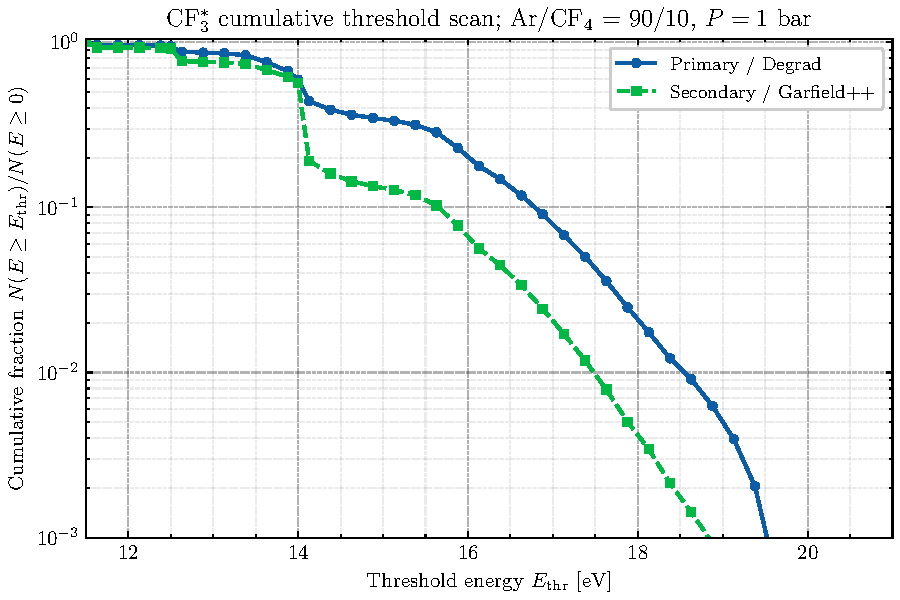
\includegraphics[width=0.99\linewidth]{cumulative/ArCF4_cumulative_CF3_cf4_10pct_1bar.pdf}
    \captionof{figure}{Poblaciones acumuladas normalizadas para $\CF_{3}$ comparando Degrad (ionización foton priamrio) y secundario (electrón en MPGD).}
    \label{fig:CF3cumulative}
\end{minipage} 

Con las simulaciones y datos experimentales del centelleo secundario únicamente para $P_{\Ar^{**}}$ y $P_{\CF_3|_{\vis,\dir}}$. Magboltz (y por ende Garfield++ y Degrad) si posee las secciones eficaces de los diferentes estados excitados. En el caso de las otras probabilidades efectivas ($P_{\Ar^{++}}$ y $P_{\CF_4^{+,*}} |_{\dir}$) no podemos desambiguar esta relación debido a la falta de conocimiento de estas secciones eficaces por excitación. 

\begin{equation}
    P_{\Ar^{**}} = P_{\Ar^{**}}^* \cdot f_{\Ar^{**}} (\varepsilon_{\Ar^{**}}) \qquad f_{\Ar^{**}} (\varepsilon_{\Ar^{**}}) = \frac{\sum_{i} \left( \theta (\epsilon_i > \varepsilon_{\Ar^{**}}) \cdot  N_{\Ar^{**}} (\varepsilon_i) \right)}{\sum_{i} N_{\Ar^{**}} (\varepsilon_i)}
 \end{equation}\begin{equation}
    \left. P_{\CF_3} \right| _{\vis,\dir} = P_{\CF_3}^* \cdot f_{\CF_3^{*}}(\varepsilon_{\CF_3^{*}})  \qquad f_{\CF_3^{*}}  (\varepsilon_{\CF_3^{*}})= \frac{\sum_{i} \left( \theta (\epsilon_i > \varepsilon_{\CF_3^{*}}) \cdot  N_{\CF_3^{*}} (\varepsilon_i) \right)}{\sum_{i} N_{\CF_3^{*}} (\varepsilon_i)}
 \end{equation}

siendo $\theta$ la función escalón y $\varepsilon_i$ la energía de cada estado. Los valores $\varepsilon_{\Ar^{**}}$ y $\varepsilon_{\CF_3^{*}}$ los límites inferioes de energía (\textit{thresholds}) para $\Ar^{**}$ y $\CF_3^{*}$ respectivamente. Así pues usaremos la notación

\begin{equation}
    N(\varepsilon) = f (\varepsilon) \cdot N
\end{equation}

El valor de límite inferior de energía que usaremos nosotros para la evaluación del os parámetros será 12.9 eV para el Ar$^{**}$ y el CF$_3^{*}$. Las excitaciones del tipo $\Ar(p)$ empiezan a partir de los 12.9 eV. Sadeghi et al \cite{Sadeghi} demuestra que las transferencias de los estados excitados tipo $p$ del Ar$^{**}$ son de un orden 10 más efectivas que las transferencias de los estados excitados tipo $s$. El buen resultado de las predicciones en el secundario permitirá evaluar la calidad de estos \textit{thresholds}. 

Este proceso no podemos efectuarlo para los estados del tercer continuo ni para $\CF_4^{*,+}$ debido al hecho de que no tenemos información de estos estados ni en Degrad ni en Garfield++, tal y como hemos advertido. Esto dificultará bastante la reproducción de los resultados en el secundario. Una mejora de las secciones eficaces experimentales de ambos gases permitiría implementar este proceso de identificación.


\subsection{Ar--CF$_4$}

Así pues, ecuaciones del ajuste (recordando que $n=p/p_0$ siendo $p$ la presión y $p_0=1$ bar y $f$ es concentración del aditivo $\CF_4$), realizadas a partir de las ecuaciones (\ref{eq:YvisCF3},\ref{eq:YuvCF4},\ref{eq:YuvAr3rd}) con las debidas correcciones son
{\small
\begin{equation*}
\begin{aligned}
\frac{Y_{\vis}}{W_I(f)}
&=
N_{\norma} \Bigg[
N_{\CF_3}(12.9\,\mathrm{eV})  \cdot P_{\CF_3^*} 
+
N_{\Ar^{**}}(12.9\,\mathrm{eV}) \cdot P_{\Ar^{**}}^*
\frac{
n f K_{\Ar^{**}Q(\CF_4)}
}{
n f K_{\Ar^{**}Q(\CF_4)}
+
n(1-f)K_{\Ar^{**}Q(\Ar)}
+
1/\tau_{\Ar^{**}}
} \Bigg]
\end{aligned}
\end{equation*}
}

\begin{equation*}
    \frac{Y_{\CF_4,\uv}}{W_I(f)} 
    =
    {N_{\norma}}
    \cdot
    P_{\CF_4^{+,*}}
    \cdot
    \bqty{
      N_{\CF_3^+}\cdot \left. P_{\CF_4^{+,*}} \right|_{\dir}
      +
      N_{\Ar^{++}}\cdot P_{\Ar^{++}}
      \pqty{
        \frac{n \cdot f \cdot K_{\Ar^{++}Q(\CF_4)}}{
        1/\tau_{\third} + n \cdot f \cdot K_{\Ar^{++}Q(\CF_4)}}
      }
    }.
\end{equation*}

\begin{equation*}
    P_{\CF_4^{+,*}}
    =
    \frac{n \cdot f \cdot K_{\text{relax}}}{
    n \cdot f \cdot K_{\text{relax}} + 1/\tau_{\text{dissc}}}
    \cdot
    \frac{1/\tau_{\uv}}{
    1/\tau_{\uv} + n \cdot f \cdot K_{\CF_4^{+,*}Q(\CF_4)}}.
\end{equation*}

\begin{equation*}
     \frac{Y_{\Ar_{\third},\uv}}{W_I(f)}
    = 0.49 \cdot
    {N_{\norma}}
    \cdot
    N_{\Ar^{++}}
    \cdot
    \pqty{
      \frac{1/\tau_{\third}}{
      1/\tau_{\third} + n \cdot f \cdot K_{\Ar^{++}Q(\CF_4)}}
    }.
\end{equation*}

\begin{equation*}
    Y_{\CF_3,\uv}
    = \left. P_{\CF_3^*}\right|_{\uv,\dir} \cdot 
    Y_{\CF_3,\vis}.    
\end{equation*} 

En el caso del tercer continuo del argón hay que añadir un factor 0.49 debido a que el 51\% de la emisión está fuera del rango de observación (recordamos que el tercer continuo emite desde el 180 hasta 250 nm). En resumen, el ultravioleta

\begin{equation}
   Y_{\uv} =Y_{\CF_4,\uv} + Y_{\Ar_{\third},\uv} + Y_{\CF_3,\uv}.
\end{equation}

Los resultados experimentales cuentan con 6 presiones (1, 2, 2.5, 3, 4 y 5 bar) y 12 concentraciones diferentes (desde 0\% a 100\% $\CF_4$)\footnote{Para el visible no vamos a usar la información de 0\% de \CFt, ya que no hay emisión en este rango y la lectura óptica es ruido principalmente.} para 1 y 4 bar, 11 concentraciones diferentes (desde 0\% a 50\% $\CF_4$) para 2, 3 y 5 bar y 1 concentración (100\% $\CF_4$) para 2.5 bar. En total son 74 valores experimentales. 

El ajuste obtenido con una $\chi^2=0.61$ muestra que nuestro modelo es compatible con los datos. En las imágenes \ref{fig:ArCF4visFit} (visible) y \ref{fig:ArCF4uvFit} (ultravioleta) representamos el resultado del ajuste. En el caso del ultravioleta representamos el 0\% de CF$_4$ en 0.001\%. 

\begin{minipage}{0.48\linewidth}
    \centering
    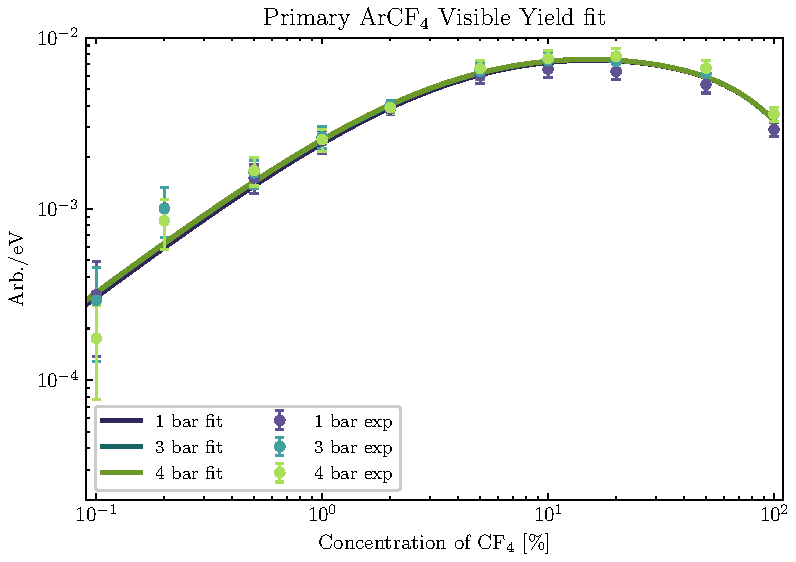
\includegraphics[width=0.99\linewidth]{primary_fit/ArCF4_visible.pdf}
    \captionof{figure}{Ajuste del rendimiento visible en Ar--CF$_4$.}
    \label{fig:ArCF4visFit}
\end{minipage} \hfill
\begin{minipage}{0.48\linewidth}
    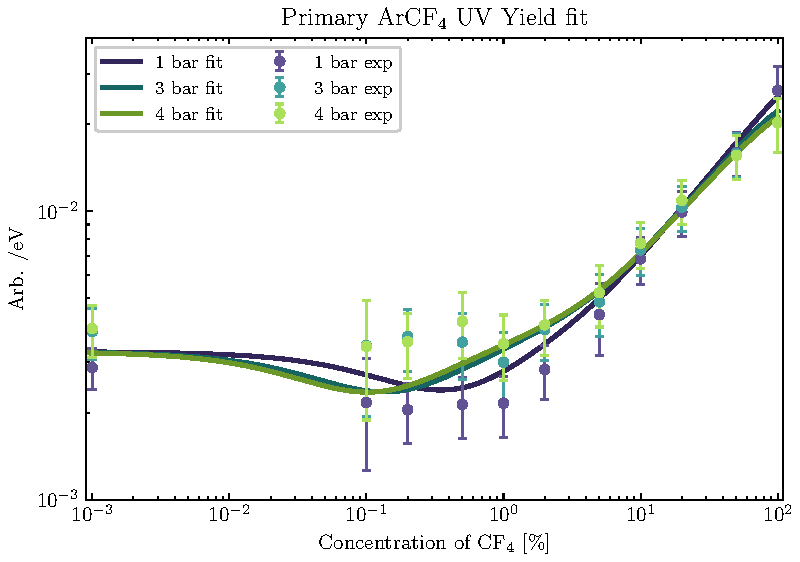
\includegraphics[width=0.99\linewidth]{primary_fit/ArCF4_uv.pdf}
    \captionof{figure}{Ajuste del rendimiento uv. en Ar--CF$_4$.}
    \label{fig:ArCF4uvFit}
\end{minipage} 

Los parámetros los representamos en la tabla \ref{tab:ArCF4_UV_VIS_toy_uncertainties}. Los parámetros del modelo primario son los resultados directos del ajuste, mientras que los parámetros del modelo primario y secundario son los parámetros capaces de describir mejor los valores del centelleo primario y secundario simultáneamente. Es decir, para predecir correctamente los ph/$e^-$ necesitamos hacer unos pequeños ajustes en la región del visible y un gran cambio de los parámetros en el caso del ultravioleta, debido a la falta de secciones eficaces para diferentes estados que impide el uso de un threshold o una diferenciación de estados .

\begin{table}[htbp]
\centering
\caption{Parámetros del ajuste primario (izquierda) y del primario \& secundario (derecha) UV/VIS en Ar--CF$_4$. Nótese las pequeñas variaciones en determinados parámetros que son necesarias para la descrición óptima del secundario y que aún mantienen una descripción del primario razonable ($\chi^2_{\mathrm{red}} \sim 2$)}
\label{tab:ArCF4_UV_VIS_toy_uncertainties}
\begin{tabular}{lcccccc}
\toprule
 & \multicolumn{3}{c}{Primario} & & \multicolumn{1}{c}{Primario \& Secundario} \\
\cmidrule(lr){2-4} \cmidrule(lr){5-6}
Parámetro & Valor & Stat. & Syst. &  &  Valor  \\
\midrule
$N_{\mathrm{norm}}$ & \num{4.46e-3} & $^{+\num{1.4e-3}}_{-\num{3.1e-4}}$ & $^{+\num{1.2e-3}}_{-\num{6.9e-6}}$ &  &  \num{4.46e-3} \\
$P_{\mathrm{CF}_3}^{*}$ & \num{6.98e-2} & $^{+\num{2.2e-3}}_{-\num{1.7e-2}}$ & $^{+\num{1.5e-3}}_{-\num{1.7e-2}}$ &  &  \num{1.39e-1}  \\
$P_{\mathrm{Ar}^{**}}^*$ & \num{1.51e-1} & $^{+\num{1.4e-2}}_{-\num{3.5e-2}}$ & $^{+\num{1.6e-3}}_{-\num{3.2e-2}}$ &  &  \num{1.21e-1} \\
$K_{\mathrm{Ar}^{**},Q(\mathrm{Ar})}$ & \num{3.9e-1} & $^{+\num{3.4e2}}_{-\num{2.5e-1}}$ & $^{+\num{1.9e-2}}_{-\num{3.7e-2}}$ &   &  \num{3.9e-1} \\
$K_{\mathrm{Ar}^{**},Q(\mathrm{CF}_4)}$ & \num{1.15e1} & $^{+\num{1e4}}_{-\num{7.1e0}}$ & $^{+\num{4.5e-1}}_{-\num{1.1e0}}$  &  & \num{1.15e1} \\
$1/(\tau_{\mathrm{disc}}K_{\mathrm{relax}})$ & \num{5.68e-3} & $^{+\num{1.4e-2}}_{-\num{1.4e-4}}$ & $^{+\num{6e-3}}_{-\num{4.8e-3}}$ &  & \num{5.68e-3} \\
$\tau_{\mathrm{UV}}K_{\mathrm{CF}_4,Q(\mathrm{CF}_4)}$ & \num{6.5e-2} & -- & -- &  &  \num{6.5e-2}   \\
$P_{\mathrm{CF}_4}|_{\mathrm{dir}}$ & \num{2.36e-1} & $^{+\num{6.7e-3}}_{-\num{5.8e-2}}$ & $^{+\num{2.4e-2}}_{-\num{3.7e-2}}$ &  & \num{3.30e-2} \\
$K_{\mathrm{Ar}^{++},Q(\mathrm{CF}_4)}$ & \num{5.0e1} & -- & -- &  & \num{5.0e1} \\
$P_{\mathrm{Ar}^{++}}$ & \num{5.19e-1} & $^{+\num{1e-1}}_{-\num{5.5e-2}}$ & $^{+\num{2.4e-2}}_{-\num{2e-2}}$ & & \num{5.19e-1}   \\
$P_{\mathrm{CF}_3}|_{\mathrm{uv,dir}}$ & \num{0.0} & $^{+\num{+4.9e-22}}_{-\num{0}}$ & $^{+\num{+2.1e-26}}_{-\num{0}}$  &  & \num{2e-1}  \\
\bottomrule
\end{tabular}
\end{table}





\subsection{Ar--CF$_4$ en el infrarrojo}

Para la emisión NIR de Ar--CF$_4$ se ajusta de forma independiente cada longitud de onda mediante
\begin{equation}
    \frac{Y_{\mathrm{IR},\lambda}}{W_I(f)} = P_{\Ar^*,\lambda} \cdot N_{\Ar^*,\lambda} \cdot \pqty{\frac{1 / \tau_{\Ar^*,\lambda}}{1 / \tau_{\Ar^*,\lambda} + n \cdot f \cdot K_{\Ar^*, Q(\Ar), \lambda} + n \cdot (1-f) \cdot K_{\Ar^*, Q(\CF_4), \lambda}} }.
\end{equation}
Aquí $P_{\Ar^*,\lambda}$ incorpora la normalización y la fracción efectiva de estados que alimenta la línea emisora. Las figuras siguientes muestran los ajustes obtenidos para las seis líneas NIR consideradas.

\begin{minipage}{0.48\linewidth}
    \centering
    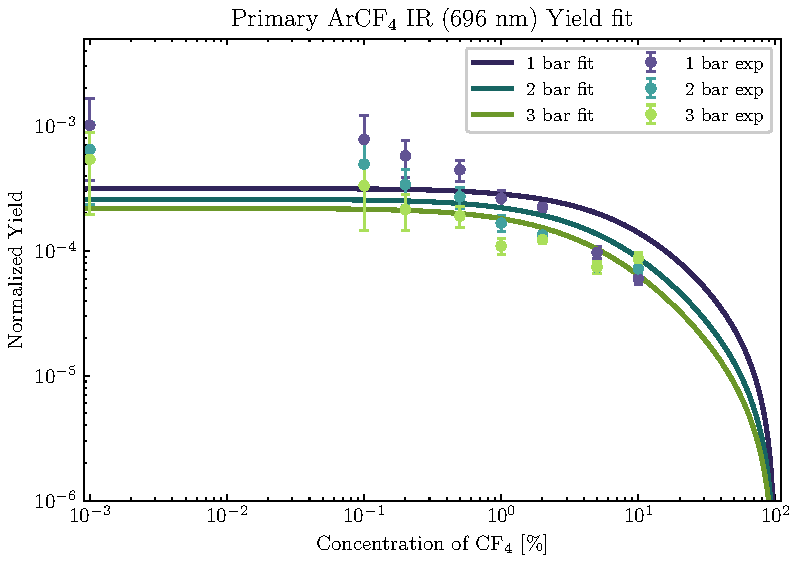
\includegraphics[width=0.99\linewidth]{primary_fit_IR/ArCF4_global_696.pdf}
    \captionof{figure}{Ajuste infrarrojo en 696 nm.}
    \label{fig:ArCF4696}
\end{minipage}
\hfill
\begin{minipage}{0.48\linewidth}
    \centering
    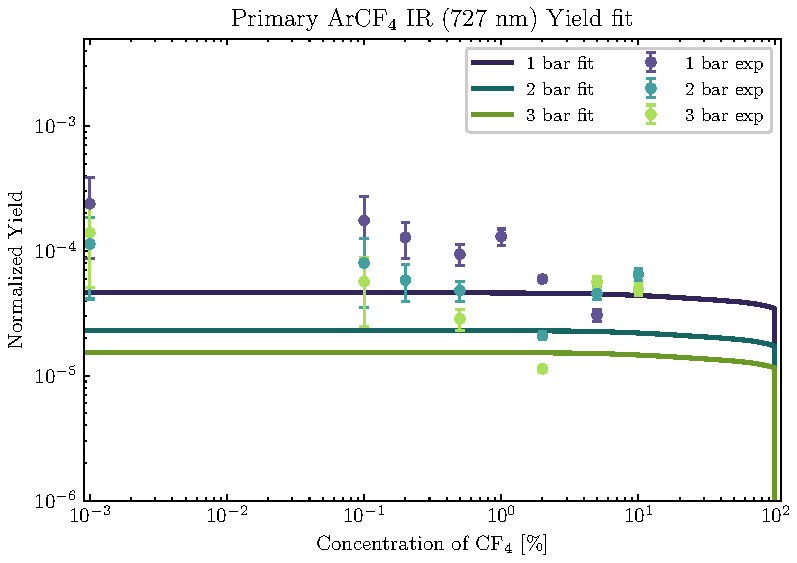
\includegraphics[width=0.99\linewidth]{primary_fit_IR/ArCF4_global_727.pdf}
    \captionof{figure}{Ajuste infrarrojo en 727 nm.}
    \label{fig:ArCF4727}
\end{minipage}


\begin{minipage}{0.48\linewidth}
    \centering
    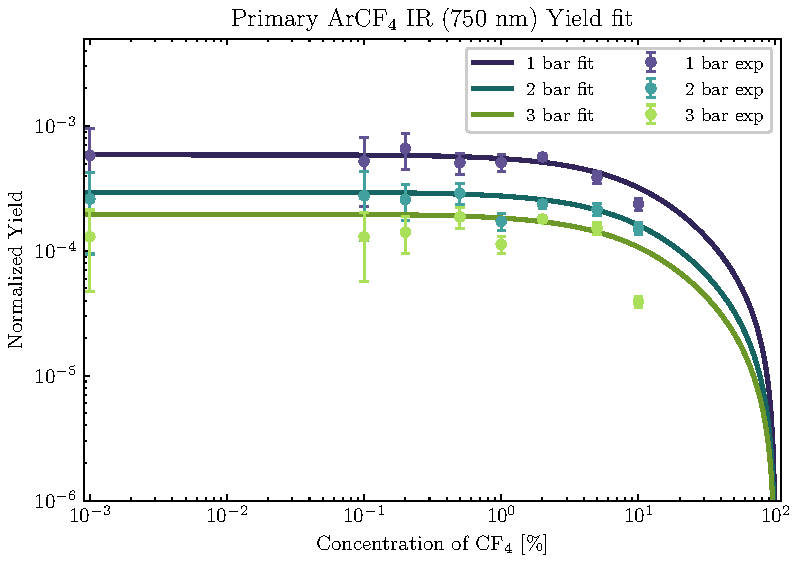
\includegraphics[width=0.99\linewidth]{primary_fit_IR/ArCF4_global_750.pdf}
    \captionof{figure}{Ajuste infrarrojo en 750 nm.}
    \label{fig:ArCF4750}
\end{minipage}
\hfill
\begin{minipage}{0.48\linewidth}
    \centering
    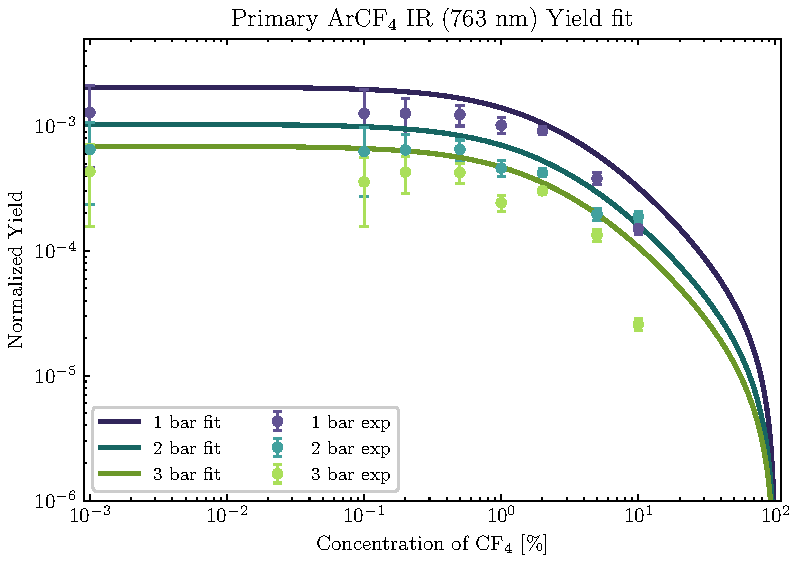
\includegraphics[width=0.99\linewidth]{primary_fit_IR/ArCF4_global_763.pdf}    \captionof{figure}{Ajuste infrarrojo en 763 nm.}
    \label{fig:ArCF4763}
\end{minipage}

\begin{minipage}{0.48\linewidth}
    \centering
    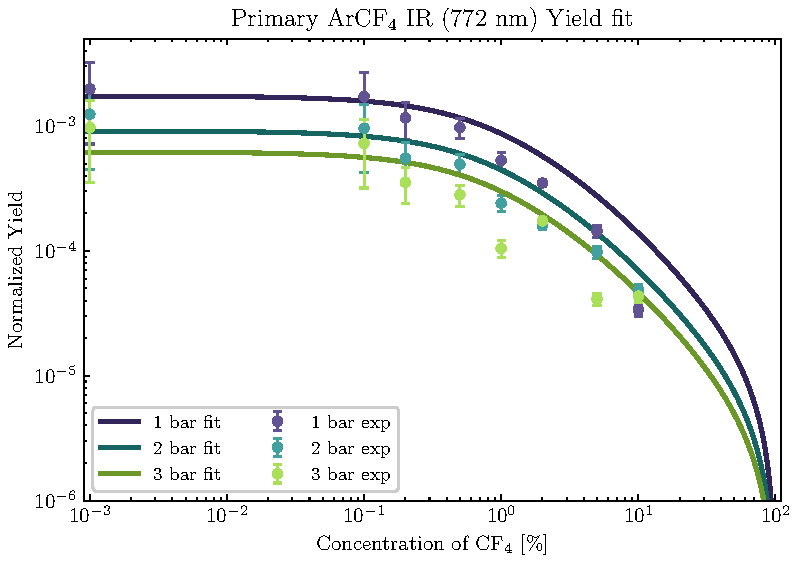
\includegraphics[width=0.99\linewidth]{primary_fit_IR/ArCF4_global_772.pdf}
    \captionof{figure}{Ajuste infrarrojo en 772 nm.}
    \label{fig:ArCF4772}
\end{minipage} \hfill
\begin{minipage}{0.48\linewidth}
    \centering
    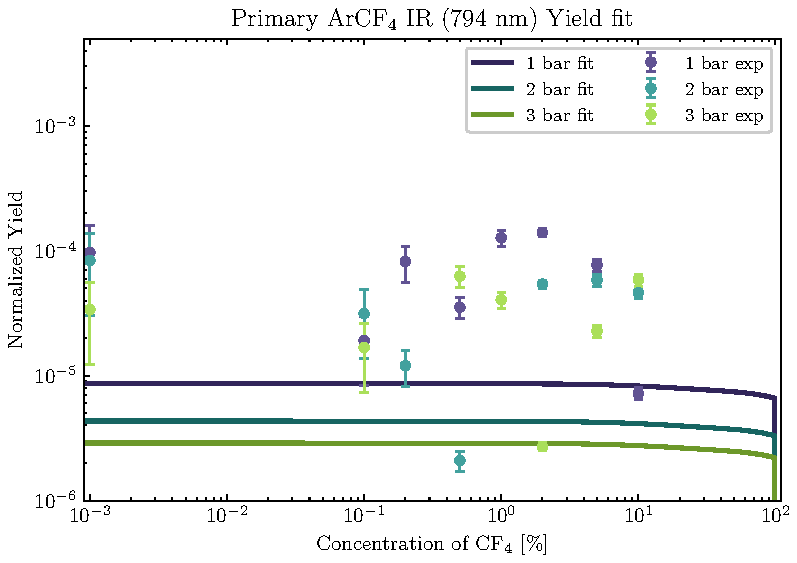
\includegraphics[width=0.99\linewidth]{primary_fit_IR/ArCF4_global_794.pdf}
    \captionof{figure}{Ajuste infrarrojo en 794 nm.}
    \label{fig:ArCF4794}
\end{minipage}

% =================================================
\section{Predicciones}
% =================================================

Con los parámetros cinéticos y las probabilidades efectivas obtenidos se realizan predicciones absolutas del centelleo primario y secundario de Ar--CF$_4$ y He--CF$_4$. Para el primario se aplican las poblaciones de Degrad; para el secundario se emplean poblaciones de avalancha producidas por Garfield++. Las predicciones se presentan en función de presión, concentración y, en el secundario, de las condiciones de amplificación.

\subsection{Predicciones en el primario}

Las predicciones primarias de Ar--CF$_4$ se expresan en fotones emitidos por energía depositada, usando en Degrad fotones incidentes de 15 keV.

\subsubsection{Predicciones absolutas ph/MeV}

En las figuras~\ref{fig:ArCF4visPrimaryPrediction} y \ref{fig:ArCF4uvPrimaryPrediction} se muestran las predicciones visibles y ultravioletas de Ar--CF$_4$ en el rango completo de concentraciones y para presiones de 1 a 5 bar. En visible se comparan con medidas absolutas de centelleo primario producido por partículas $\alpha$ a 1 bar \cite{amedo2023observation} y, para CF$_4$ puro, con \cite{lehaut2015scintillation}.

\begin{minipage}{0.48\linewidth}
    \centering
    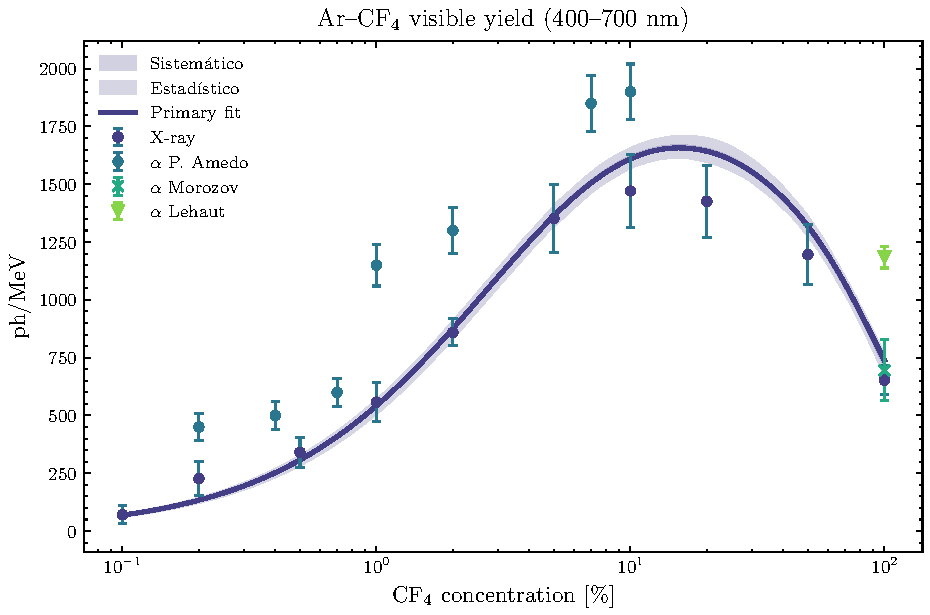
\includegraphics[width=0.99\linewidth]{primary_prediction/ArCF4_bands_vis_toy_stat_syst.pdf}
    \captionof{figure}{Rendimiento de centelleo primario absoluto visible en $\Ar-\CF_4$, comparado con datos experimentales.}
    \label{fig:ArCF4visPrimaryPrediction}
\end{minipage}
\hfill
\begin{minipage}{0.48\linewidth}
    \centering
    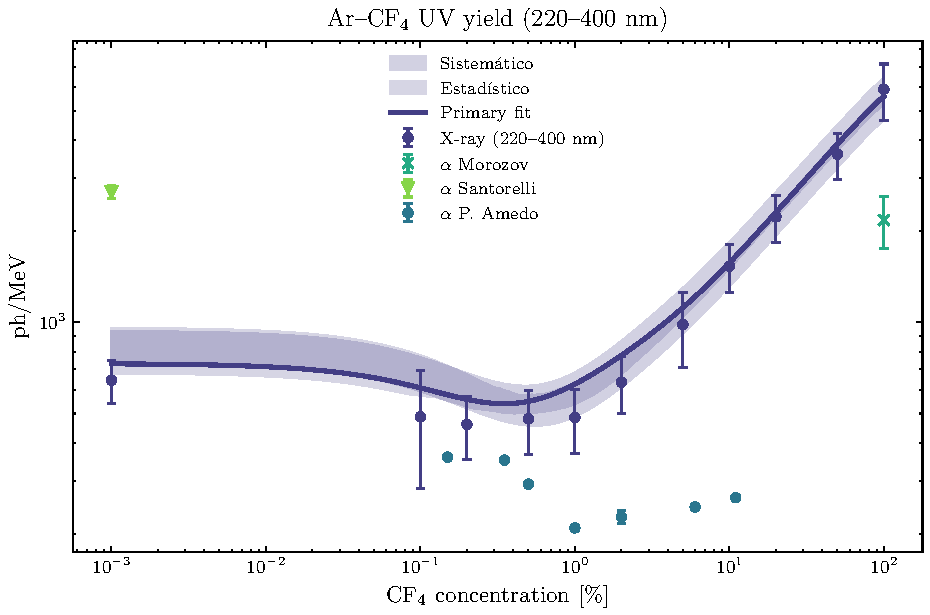
\includegraphics[width=0.99\linewidth]{primary_prediction/ArCF4_bands_uv_toy_stat_syst.pdf}
    \captionof{figure}{Rendimiento de centelleo primario absoluto ultravioleta en $\Ar-\CF_4$, comparado con datos experimentales.}
    \label{fig:ArCF4uvPrimaryPrediction}
\end{minipage}

La figura~\ref{fig:ArCF4IrPrimaryPrediction} muestra la predicción absoluta de la emisión NIR de Ar--CF$_4$ para concentraciones entre 0.01\% y 100\% y presiones de 1 a 5 bar.

\begin{figure}[h!]
    \centering
    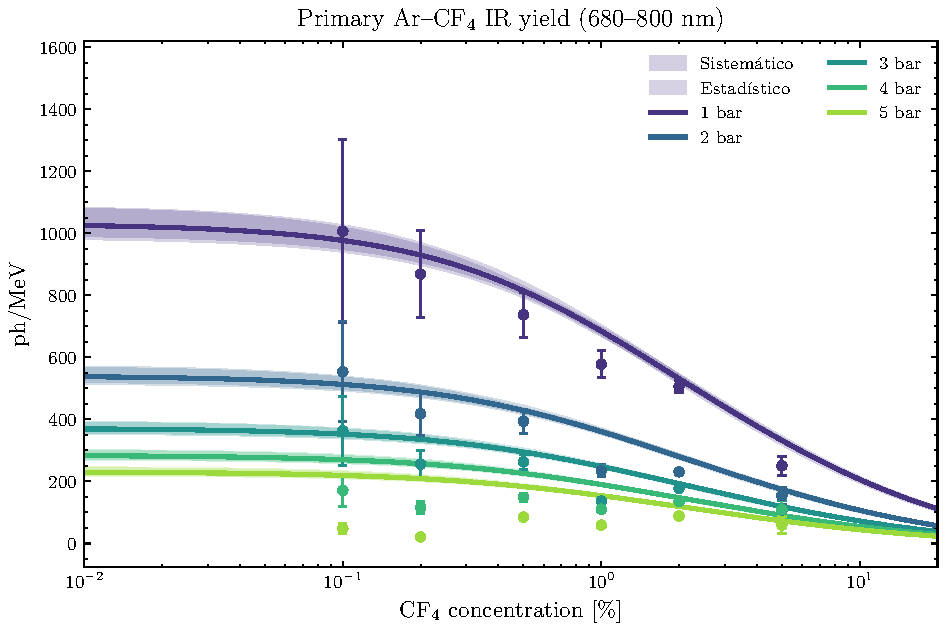
\includegraphics[width=0.62\linewidth]{primary_prediction/ArCF4_IR_total_bands_toy_stat_syst.pdf}
    \caption{Rendimiento de centelleo primario absoluto NIR en $\Ar-\CF_4$.}
    \label{fig:ArCF4IrPrimaryPrediction}
\end{figure}

\subsubsection{Espectros}

Para generar espectros emitidos se pondera cada componente de rendimiento absoluto con una función de densidad de probabilidad asociada a su pico. Usando gaussianas centradas en las longitudes de emisión discutidas en la sección~\ref{sec:experimental_espectra},
\begin{equation}
    Y(\lambda, f_{\CF_4}, p) = \sum_i Y_i(f_{\CF_4}, p)\, \mathrm{gauss}(\lambda;\, \mu=\lambda_i,\sigma=\sigma_i).
\end{equation}
La figura~\ref{fig:ArCF4PrimarySpectra} presenta los espectros predichos en el intervalo 200--800 nm para distintas concentraciones y presiones.

\begin{figure}[h!]
    \centering
    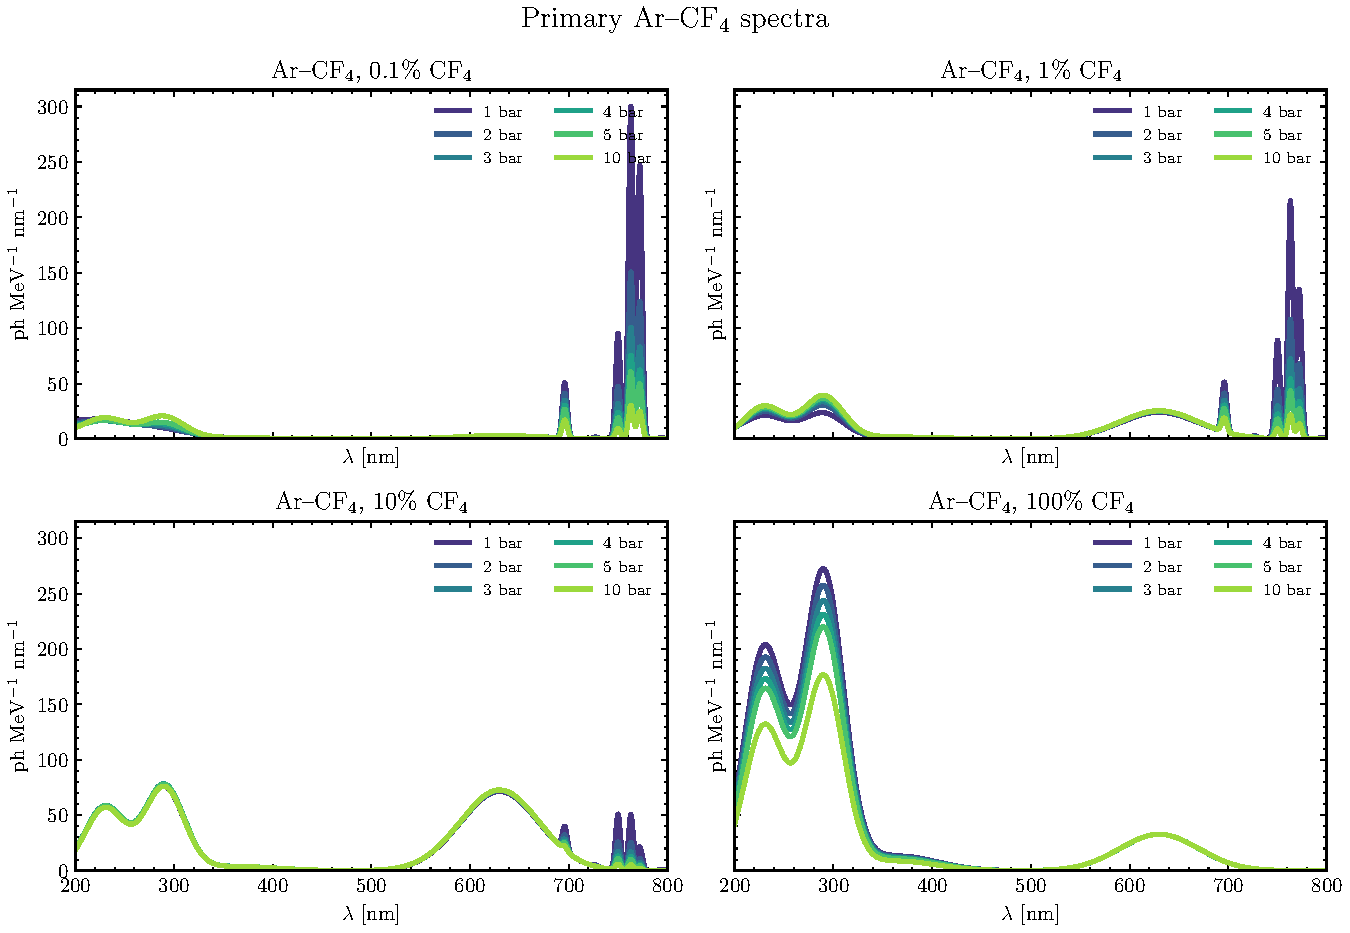
\includegraphics[width=0.9\linewidth]{predicted_spectra/ArCF4_concentration_ph_MeV_nm.pdf}
    \caption{Espectros de $\Ar-\CF_4$ predichos en función de la concentración y la presión en el rango 200--800 nm.}
    \label{fig:ArCF4PrimarySpectra}
\end{figure}

\subsection{Predicciones en el secundario}

Los GEMs, FAT-GEMs y TH-GEMs son tres de las estructuras MPGDs más utilizadas para producir avalanchas electrónicas controladas en detectores gaseosos. Sus condiciones típicas de operación se resumen en la tabla~\ref{tab:mgpd}. Aunque estas estructuras presentan diferencias geométricas muy marcadas —desde espesores del orden de decenas de micras en los GEM hasta varios milímetros en los FAT-GEM—, todas ellas comparten una misma idea física: concentrar campos eléctricos intensos en regiones pequeñas para favorecer la multiplicación electrónica y, simultáneamente, la producción de estados excitados responsables del centelleo secundario.

Estas diferencias geométricas son importantes porque modifican directamente la longitud efectiva de la avalancha, el número de colisiones electrón--gas y la relación entre ionización, excitación y pérdidas no radiativas. En una estructura fina, como un GEM convencional, la avalancha se desarrolla en una distancia corta y en campos muy altos. En cambio, en un TH-GEM o en un FAT-GEM la región de amplificación es más extensa, por lo que un electrón puede acumular un número mayor de colisiones antes de abandonar la zona activa. Esto hace que, para una ganancia electrónica comparable, las estructuras más gruesas puedan producir una cantidad mayor de fotones por electrón de avalancha, especialmente cuando el campo reducido $E/p$ se sitúa en una región favorable para la excitación.

\begin{table}[h!]
\centering
\begin{tabular}{ccc}
\toprule
MPGD & Thickness [$\mu$m] & Electric field [kV/cm]  \\
\midrule
GEMs     & 50--100     & 50--110  \\
TH-GEMs  & 300--600    & 20--50   \\
FAT-GEMs & 4500--5500  & 10--30   \\
\bottomrule
\end{tabular}
\caption{Características geométricas y rangos de operación típicos de diferentes MPGDs \cite{williams2024fatgems,azevedo2016thgem,fraga2003the}.}
\label{tab:mgpd}
\end{table}

En esta sección se estudia la predicción del centelleo secundario en mezclas $\Ar-\CF_4$ y $\He-\CF_4$, expresado en fotones por electrón de avalancha, ph/e$^-$. La estrategia es la misma que en el resto del trabajo: separar la producción microscópica de poblaciones excitadas, obtenida con Garfield++, de la evolución cinética posterior de dichas especies, descrita mediante el modelo desarrollado en la sección~\ref{Sec:model_kin}. La diferencia fundamental respecto al primario es que ahora las poblaciones no proceden de una interacción inicial de rayos X o partículas $\alpha$, sino del desarrollo de una avalancha electrónica en una región de campo intenso.

El objetivo principal de estas predicciones no es únicamente reproducir unos puntos experimentales concretos, sino comprobar si los parámetros obtenidos en el primario pueden ser transferidos al régimen de avalancha. Esta comprobación es muy exigente: el campo eléctrico modifica la distribución de energía de los electrones, la frecuencia relativa de excitaciones e ionizaciones, y la importancia de los umbrales energéticos de cada canal. Por tanto, un buen acuerdo en el secundario indicaría que el modelo no solo ajusta datos primarios, sino que captura de manera razonable la relación entre poblaciones microscópicas y emisión óptica.

\subsubsection{Comparación con datos experimentales}

En las figuras~\ref{fig:ArCF4_sec_VIS}, \ref{fig:HeCF4_sec_VIS}, \ref{fig:LIP_UV} y \ref{fig:ArCF4_sec_IR} se comparan las predicciones del modelo con datos experimentales disponibles de centelleo secundario. A lo largo de estas figuras se emplea la siguiente convención: los puntos cerrados corresponden a estimaciones indirectas del rendimiento óptico, obtenidas a partir de magnitudes experimentales intermedias o de conversiones auxiliares, mientras que los puntos abiertos, blancos por dentro, corresponden a estimaciones experimentales directas del número de fotones producidos por electrón de avalancha. Esta distinción es importante, ya que las estimaciones indirectas pueden arrastrar incertidumbres adicionales asociadas a la ganancia, la eficiencia óptica, la normalización o el procedimiento de reconstrucción.

\begin{figure}[h!]
\centering
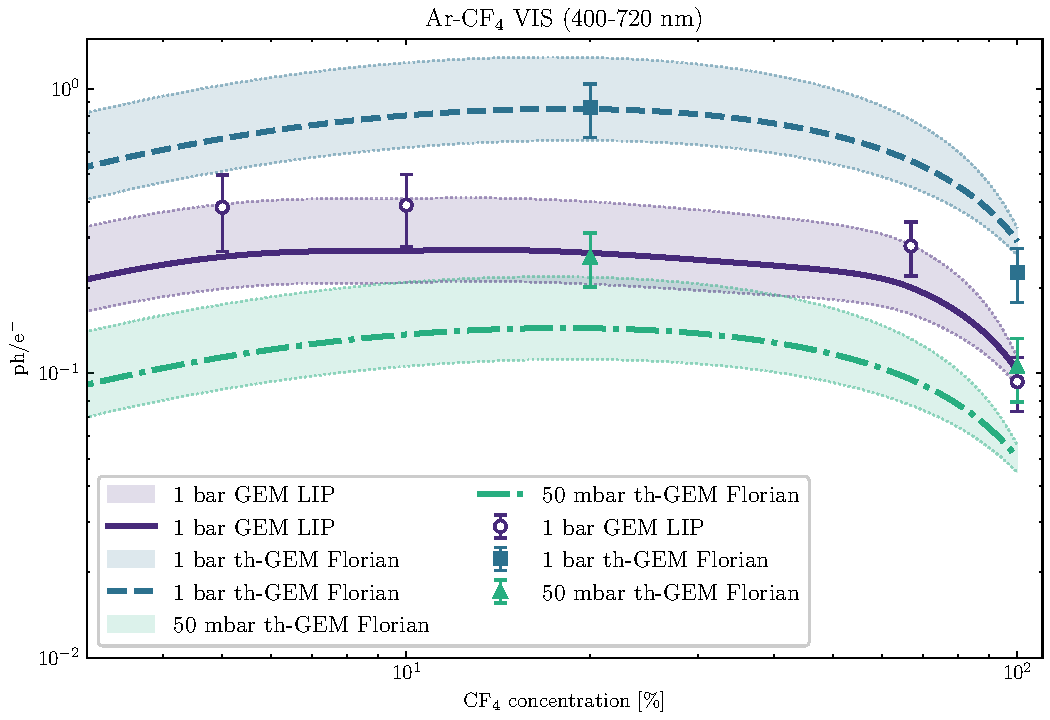
\includegraphics[width=0.9\linewidth]{secondary_prediction/ArCF4_VIS_comparation.pdf}
\caption{Predicción del centelleo secundario visible de $\Ar-\CF_4$ comparada con datos experimentales. Los puntos cerrados representan estimaciones indirectas y los puntos abiertos estimaciones directas. La banda muestra la variación asociada a los esquemas de parámetros considerados para la extrapolación al secundario.}
\label{fig:ArCF4_sec_VIS}
\end{figure}

La figura~\ref{fig:ArCF4_sec_VIS} muestra la predicción de la emisión visible en $\Ar-\CF_4$, dominada por la emisión del $\CF_3^*$ alrededor de 630 nm. Esta es una de las regiones más relevantes desde el punto de vista instrumental, ya que cae en una ventana espectral accesible para cámaras, SiPMs y fotodetectores convencionales. En este caso, la banda no representa una incertidumbre puramente estadística del ajuste primario, sino la variación entre los distintos esquemas de identificación de parámetros discutidos previamente. En particular, los parámetros efectivos más sensibles son los asociados a la contribución de los estados $\Ar^{**}$ y a la producción directa de especies emisoras de CF$_4$/CF$_3$. Dicho de otro modo, la anchura de la banda refleja hasta qué punto la predicción secundaria depende de cómo se traduzcan las poblaciones simuladas por Garfield++ en poblaciones realmente centelleadoras.

En las predicciones visible y ultravioleta de $\Ar-\CF_4$, así como en las comparaciones con $\He-\CF_4$, se incluyen tres curvas de referencia: la extrapolación directa de los parámetros del primario, la curva recomendada y la curva que proporciona la mejor descripción conjunta de primario y secundario. La banda se construye a partir de estas tres posibilidades. Esta elección es más apropiada que una banda estadística local, porque en estas regiones la incertidumbre dominante no procede únicamente del ajuste numérico, sino de la identificación física de qué fracción de las poblaciones $N_{\Ar^{**}}$, $N_{\CF_3^*}$ o $N_{\CF_4^{+,*}}$ contribuye realmente al canal radiativo observado. En el visible, esta identificación puede realizarse parcialmente mediante umbrales energéticos, como se discutió en la sección anterior. En el ultravioleta, sin embargo, la situación es más delicada, ya que no se dispone de una separación completa de los estados precursores del tercer continuo ni de los estados $\CF_4^{+,*}$ en las secciones eficaces usadas por Degrad/Garfield++.

\begin{figure}[h!]
\centering
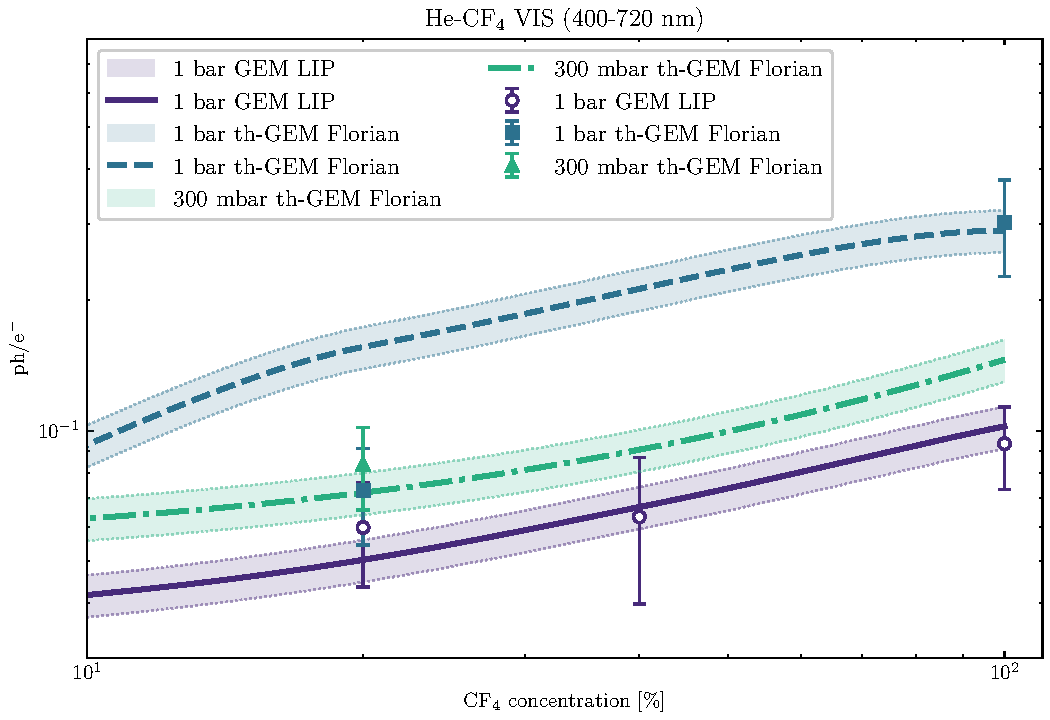
\includegraphics[width=0.9\linewidth]{secondary_prediction/HeCF4_VIS_comparation.pdf}
\caption{Predicción del centelleo secundario en $\He-\CF_4$. Al no existir transferencia energética desde el gas noble hacia el CF$_4$ en el rango espectral estudiado, esta comparación constituye una prueba directa de los parámetros asociados a la emisión propia del CF$_4$.}
\label{fig:HeCF4_sec_VIS}
\end{figure}

La comparación con $\He-\CF_4$, mostrada en la figura~\ref{fig:HeCF4_sec_VIS}, es especialmente importante. En esta mezcla no se espera un mecanismo de \textit{wavelength shifting} equivalente al de $\Ar-\CF_4$, ya que el helio no alimenta de forma eficiente las especies emisoras consideradas en el rango 200--800 nm. Por tanto, la emisión observada debe proceder esencialmente de la producción directa de especies de CF$_4$, principalmente $\CF_4^{+,*}$ y $\CF_3^*$. El buen acuerdo obtenido en esta mezcla refuerza de manera notable la interpretación física del modelo: los parámetros directos del CF$_4$ no parecen ser únicamente un ajuste efectivo de la mezcla $\Ar-\CF_4$, sino que poseen capacidad predictiva en un gas base distinto, con secciones eficaces, transporte electrónico y distribución de energía diferentes.

Este resultado es uno de los puntos más fuertes del trabajo. La mezcla $\He-\CF_4$ funciona como una comprobación externa del modelo, porque elimina buena parte de la complejidad asociada a las transferencias desde el argón. Si, aun así, la predicción describe razonablemente el centelleo secundario, entonces el esquema de separación entre producción microscópica y cinética radiativa gana credibilidad. En particular, indica que el modelo no está simplemente reproduciendo una tendencia empírica de $\Ar-\CF_4$, sino capturando una parte transferible de la física del CF$_4$ como gas centelleador.

\begin{figure}[h!]
\centering
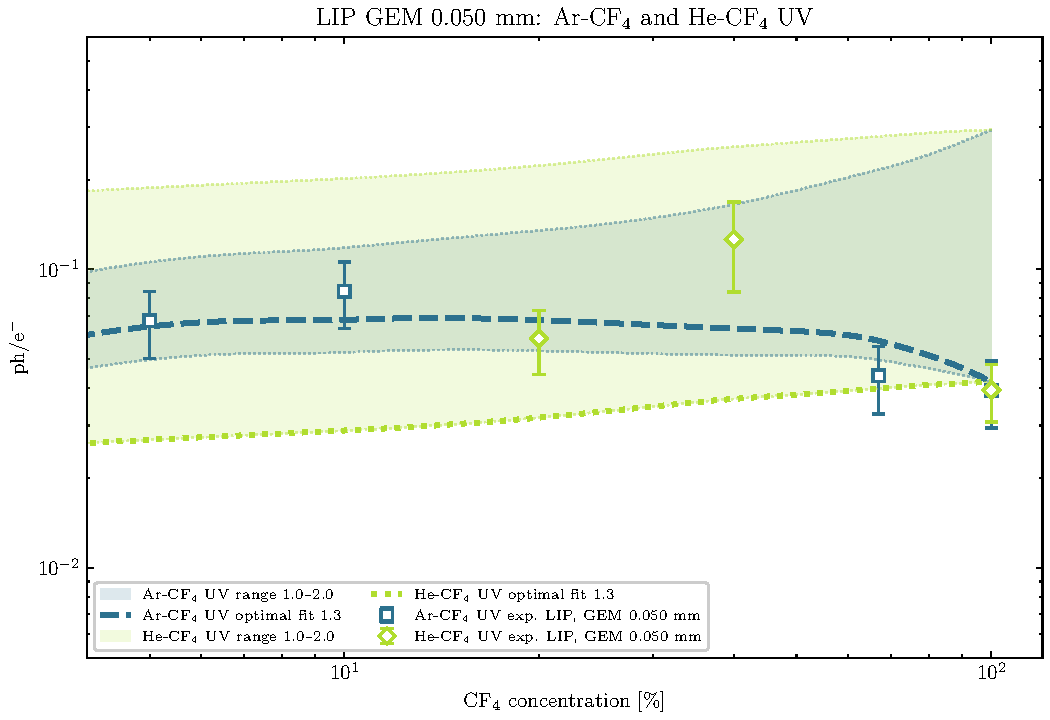
\includegraphics[width=0.9\linewidth]{secondary_prediction/LIP_UV.pdf}
\caption{Predicción del centelleo secundario ultravioleta en mezclas con CF$_4$. La descripción es razonable en el régimen de operación principal, aunque a baja presión el esquema de umbrales pierde validez y la predicción se vuelve menos robusta.}
\label{fig:LIP_UV}
\end{figure}

La figura~\ref{fig:LIP_UV} presenta la comparación en el ultravioleta. En esta región el modelo reproduce de forma cualitativa la escala y la tendencia general de los datos, pero aparecen desviaciones más claras, especialmente a baja presión. Este comportamiento es esperable. La emisión ultravioleta involucra varias contribuciones superpuestas: la emisión de $\CF_4^{+,*}$, la posible contribución UV del $\CF_3^*$ y la componente asociada al tercer continuo del argón. A diferencia del visible, donde el umbral de 12.9 eV proporciona una forma razonable de seleccionar las excitaciones relevantes de $\Ar^{**}$ y $\CF_3^*$, en el UV no se dispone de una descomposición microscópica equivalente para todos los precursores. Por tanto, el modelo debe usar parámetros efectivos más globales.

A baja presión, además, el esquema basado en umbrales se vuelve menos fiable. Al disminuir la presión, aumenta la longitud libre media y cambia la forma en la que los electrones ganan energía entre colisiones. La distribución energética de la avalancha puede poblar de manera diferente los estados excitados respecto al régimen para el que se ha calibrado el modelo. Como consecuencia, una selección fija de estados por encima de un cierto threshold deja de representar correctamente la fracción real de excitaciones que terminan produciendo luz. Esta es probablemente la razón principal por la que la predicción UV empeora en el régimen de baja presión. No debe interpretarse como un fallo global del modelo cinético, sino como una limitación concreta de la identificación efectiva de estados emisores cuando cambia de forma sustancial la distribución microscópica de la avalancha.

\begin{figure}[h!]
\centering
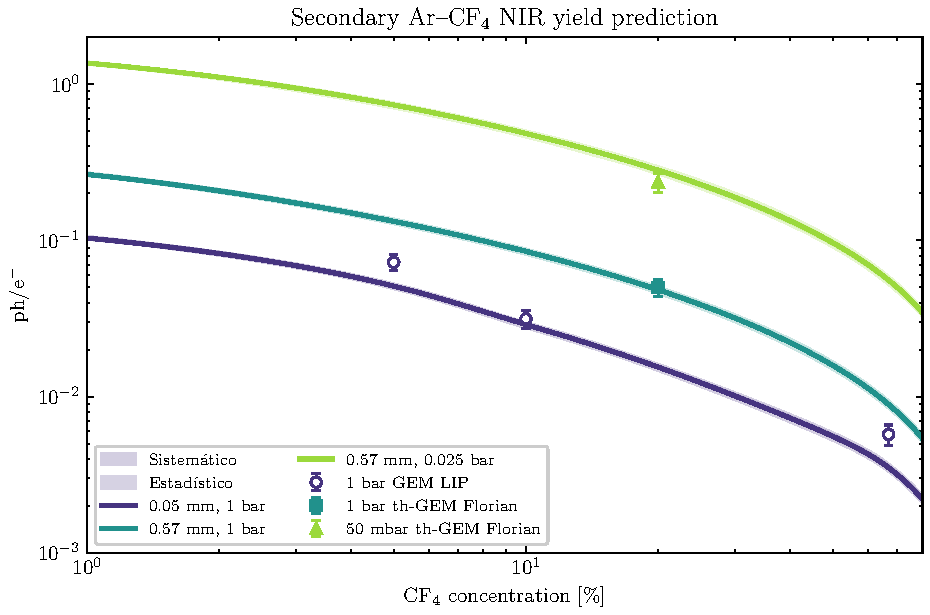
\includegraphics[width=0.9\linewidth]{secondary_prediction/ArCF4_IR_secondary_with_bands.pdf}
\caption{Predicción del centelleo secundario infrarrojo cercano de $\Ar-\CF_4$. En este caso no se realiza un reajuste específico al secundario: la banda procede directamente de la propagación de las incertidumbres estadísticas y sistemáticas del ajuste primario IR.}
\label{fig:ArCF4_sec_IR}
\end{figure}

La predicción infrarroja de la figura~\ref{fig:ArCF4_sec_IR} tiene una naturaleza distinta a las anteriores. En el NIR no se han retocado parámetros para describir el secundario. Las líneas entre 680 y 800 nm proceden de transiciones atómicas del argón, y el modelo empleado es una extrapolación directa del ajuste primario IR descrito en la sección~\ref{subbsec:kinArIR}. Por ello, la banda mostrada no se construye con las tres curvas de parámetros usadas en el visible y el UV, sino propagando las incertidumbres estadísticas y sistemáticas del primario al rendimiento secundario. Esta banda es relativamente pequeña, especialmente al representarla en escala logarítmica, porque no incluye incertidumbres adicionales asociadas a la normalización experimental secundaria, a la ganancia o a la eficiencia óptica. Representa únicamente la incertidumbre heredada de los parámetros cinéticos del modelo IR primario.

El buen acuerdo en el infrarrojo es, por tanto, especialmente significativo. A diferencia del visible de $\Ar-\CF_4$, donde se introducen ajustes asociados a la identificación de $P_{\Ar^{**}}$ y de las poblaciones emisoras de CF$_4$/CF$_3$, el NIR constituye una predicción mucho más directa. El hecho de que la escala absoluta y la dependencia con la concentración se reproduzcan razonablemente sugiere que las poblaciones de argón excitado simuladas por Garfield++ y el modelo de quenching radiativo-colisional capturan de forma correcta la física dominante. Además, el IR resulta particularmente relevante a bajas concentraciones de CF$_4$, donde la mezcla sigue estando dominada por argón y las líneas NIR pueden aportar una señal óptica no despreciable incluso cuando la emisión molecular del aditivo todavía no es máxima. Esta característica puede ser útil instrumentalmente, ya que ofrece una ventana espectral complementaria a la emisión visible y UV del CF$_4$.

\subsubsection{Dependencia con la concentración y la presión}

Una vez validada la escala general del modelo frente a datos experimentales, se estudia la dependencia del centelleo secundario con la concentración de CF$_4$ y la presión. Las figuras~\ref{fig:GEM} y \ref{fig:th-GEM} muestran predicciones en un rango de 0.05 bar a 10 bar para el TH-GEM y de 0.2 bar 10 bar para el GEM  En el caso de los GEM y TH-GEM se elige una ganancia electrónica fija de 100, es decir, calculamos el campo eléctrico para la presión y gap elegidos, a través de un ajuste de los coeficientes towsend obtenidos a partir de simulaciones. De este modo se explica que el punto de baja presión del GEM sea 0.2 bar y no 0.05 bar, ya que en las condiciones de 0.05 bar no existe ningún campo que permita un coeficiente towsend que alcannce la ganancia 100 para dicho gap de 0.050 mm. 

Así pues, representamos condiciones típicas de GEM y TH-GEM, incluyendo simultáneamente la contribución visible y la infrarroja. Estas figuras permiten comparar cómo cambia la señal óptica al modificar la geometría efectiva de amplificación y el régimen de campo.

\begin{figure}[h!]
\centering
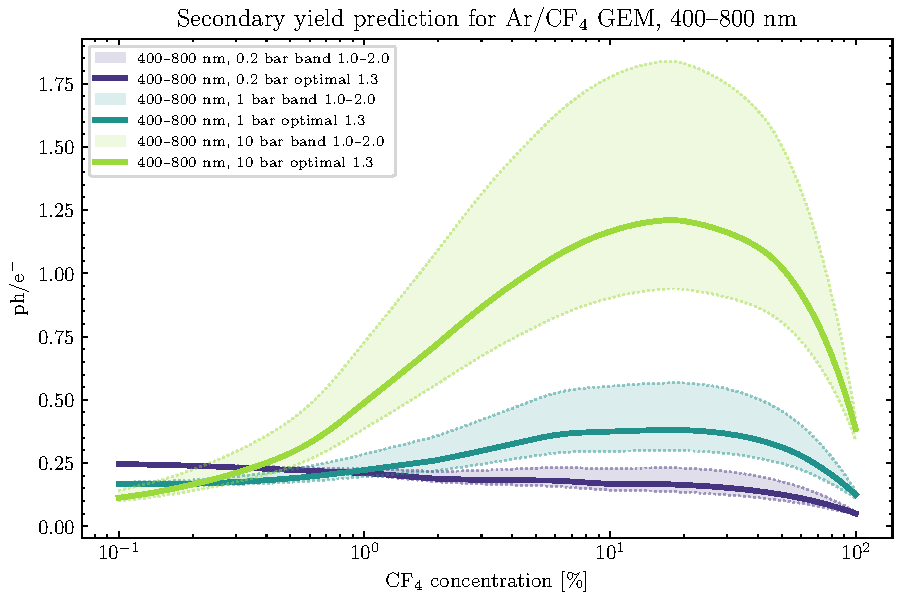
\includegraphics[width=0.9\linewidth]{secondary_prediction/paper_v2_ArCF4_gem_VIS_IR.pdf}
\caption{Predicción del centelleo secundario visible e infrarrojo de $\Ar-\CF_4$ para condiciones representativas de una geometría tipo GEM. La banda refleja la variación asociada a los parámetros efectivos $P_{\Ar^{**}}$ y a la producción directa de especies emisoras de CF$_4$/CF$_3$.}
\label{fig:GEM}
\end{figure}

En geometrías tipo GEM, figura~\ref{fig:GEM}, la región de amplificación es corta y el campo eléctrico necesario para alcanzar una ganancia apreciable es elevado. En estas condiciones, la producción de excitaciones se concentra en una distancia pequeña. La señal visible aumenta de forma clara al introducir pequeñas cantidades de CF$_4$, debido a la transferencia desde estados excitados del argón y a la producción directa de especies de CF$_4$. Sin embargo, a concentraciones más altas aparecen mecanismos competitivos: el quenching, el attachment y la redistribución de la energía electrónica modifican la eficiencia de producción de luz. Como resultado, el rendimiento óptico no crece de forma indefinida con la concentración, sino que presenta regiones óptimas.

La presión introduce un efecto igualmente importante. En los rangos de operación considerados, las presiones más altas pueden favorecer una mayor producción óptica por electrón de avalancha. Esto se debe a que, para condiciones de ganancia y geometría comparables, el campo reducido efectivo $E/p$ puede situarse en una región donde aumenta la frecuencia de colisiones excitadoras respecto a un régimen excesivamente energético. En términos simples, al aumentar la presión crece el número de moléculas disponibles por unidad de longitud y se reduce la distancia media entre colisiones. Si el campo es suficiente para mantener la avalancha, esta mayor densidad colisional puede traducirse en un número mayor de excitaciones y, por tanto, en más fotones producidos por electrón. Este comportamiento es particularmente atractivo para detectores de procesos raros, donde interesa maximizar la señal óptica sin empujar la estructura hacia regímenes de descarga o inestabilidad.

\begin{figure}[h!]
\centering
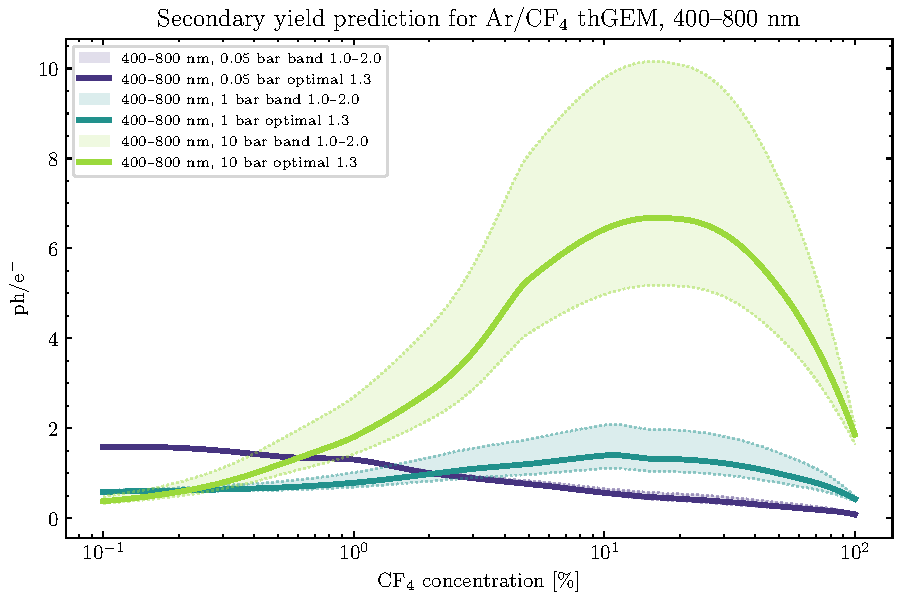
\includegraphics[width=0.9\linewidth]{secondary_prediction/paper_v2_ArCF4_thgem_VIS_IR.pdf}
\caption{Predicción del centelleo secundario visible e infrarrojo de $\Ar-\CF_4$ para condiciones representativas de una geometría tipo TH-GEM. La mayor longitud efectiva de avalancha favorece un incremento del rendimiento óptico frente a estructuras más finas.}
\label{fig:th-GEM}
\end{figure}

La figura~\ref{fig:th-GEM} muestra el caso de una geometría tipo TH-GEM. El aumento del espesor respecto a un GEM convencional permite una región de avalancha más extensa y, por tanto, un mayor número de colisiones acumuladas por electrón. Esto se refleja en un incremento del rendimiento óptico esperado. Desde el punto de vista del diseño de detectores, este resultado es muy relevante: no solo importa alcanzar una ganancia electrónica alta, sino también producir la mayor cantidad posible de luz por electrón amplificado. Dos estructuras con ganancias similares pueden tener rendimientos ópticos diferentes si la historia microscópica de la avalancha no es la misma.

Esta observación es especialmente sugerente para FAT-GEMs. Al tratarse de estructuras todavía más gruesas, capaces de operar con campos más moderados y regiones de amplificación de varios milímetros, es razonable esperar una producción óptica aún mayor, siempre que la ganancia permanezca estable y no aparezcan pérdidas dominantes por attachment, quenching excesivo o descargas. En este sentido, el modelo apunta a que las estructuras gruesas pueden ser candidatas especialmente interesantes para lectura óptica en TPCs gaseosas, donde se busca una señal luminosa intensa, extendida y compatible con sensores externos.

En las figuras~\ref{fig:GEM} y \ref{fig:th-GEM} las bandas asociadas al visible siguen teniendo la misma interpretación que en la comparación inicial con datos: reflejan la incertidumbre entre los esquemas de parámetros efectivos, principalmente los relacionados con $P_{\Ar^{**}}$ y con la producción directa de especies emisoras de CF$_4$/CF$_3$. Es decir, la banda no debe interpretarse como una fluctuación estadística local, sino como la variación física asociada a la identificación de qué fracciones de las poblaciones simuladas son realmente radiativas en el secundario. En cambio, la contribución IR se comporta como una predicción más directa, ya que procede de parámetros ajustados en el primario y propagados al secundario sin ajuste adicional.

Un resultado importante de estas predicciones es el papel del infrarrojo a baja concentración de CF$_4$. En esta región, la mezcla sigue estando dominada por argón y las líneas NIR conservan una contribución relevante. Al aumentar la concentración de CF$_4$, las emisiones moleculares visibles y UV ganan peso, pero también aumenta el quenching de los estados de argón responsables del IR. Por tanto, el NIR aparece como una señal especialmente útil en mezclas pobres en aditivo, mientras que la emisión visible del CF$_4$ domina en regiones donde la transferencia y la producción directa de especies moleculares son más eficientes. Esta complementariedad espectral puede ser muy valiosa para detectores ópticos, ya que permite seleccionar la ventana de lectura según la mezcla, la presión y la estructura de amplificación.

\subsubsection{Dependencia con la concentración y el campo eléctrico}

La figura~\ref{fig:ArCF4_sec_vsE_1percentCF4} muestra la dependencia del rendimiento visible e infrarrojo con el campo eléctrico para una concentración fija de 1\% de CF$_4$. Este tipo de representación es especialmente útil porque conecta directamente el modelo con una variable de operación del detector. Mientras que la concentración y la presión definen la composición y la densidad del gas, el campo eléctrico determina la energía media adquirida por los electrones entre colisiones y, por tanto, la probabilidad relativa de excitación, ionización y attachment.

\begin{figure}[h!]
\centering
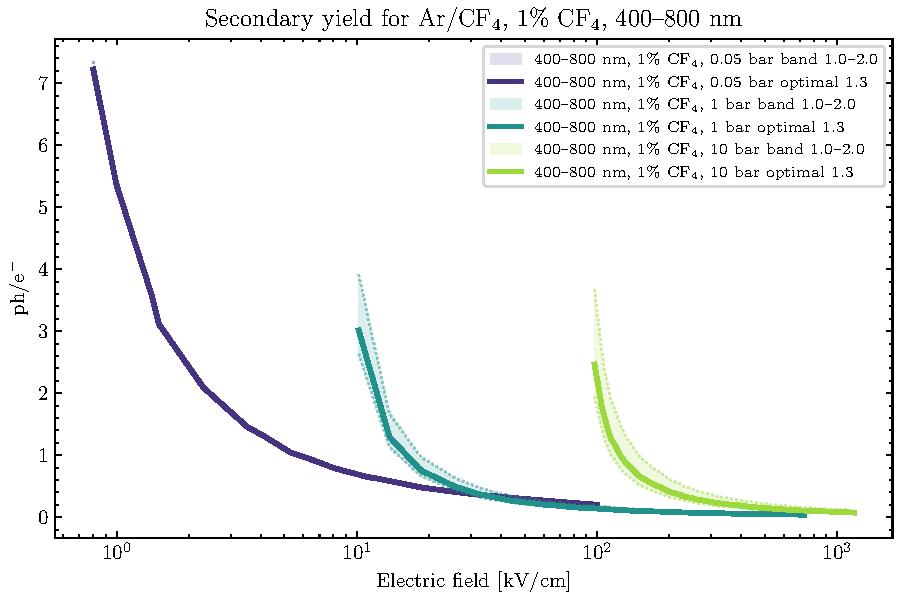
\includegraphics[width=0.9\linewidth]{secondary_prediction/paper_v2_ArCF4_VIS_IR_vsE_1percentCF4.pdf}
\caption{Predicción del centelleo secundario visible e infrarrojo de $\Ar-\CF_4$ en función del campo eléctrico para una concentración de 1\% de CF$_4$.}
\label{fig:ArCF4_sec_vsE_1percentCF4}
\end{figure}

A campos bajos, la energía adquirida por los electrones puede ser insuficiente para poblar eficientemente los estados excitados responsables de la emisión. Al aumentar el campo, crece la probabilidad de superar los umbrales de excitación e ionización, de modo que tanto la ganancia como el número de fotones por electrón pueden aumentar de forma significativa. Sin embargo, este crecimiento no debe interpretarse como indefinido. A campos muy elevados, una fracción creciente de la energía electrónica puede dirigirse hacia ionización, attachment o canales no radiativos, y además la estabilidad eléctrica de la estructura se vuelve más crítica. Por ello, la región instrumentalmente más interesante no es necesariamente la de campo máximo, sino aquella donde la producción óptica es alta y la operación del detector sigue siendo estable.

En el caso de mezclas con pequeñas concentraciones de CF$_4$, la competencia entre visible e IR resulta especialmente ilustrativa. El visible se beneficia de la presencia del aditivo molecular y de la transferencia desde estados excitados del argón, mientras que el IR refleja de forma más directa la supervivencia radiativa de estados excitados atómicos del argón. Por tanto, al modificar el campo eléctrico se modifica también el balance entre ambas ventanas espectrales. Este hecho abre la posibilidad de optimizar el detector no solo en términos de ganancia electrónica, sino también en términos de composición espectral de la luz emitida.

\subsubsection{Discusión física e implicaciones instrumentales}

Los resultados obtenidos en el secundario muestran un grado de acuerdo notable con los datos disponibles, especialmente si se tiene en cuenta que gran parte de las predicciones se obtienen a partir de parámetros ajustados en el primario y poblaciones microscópicas simuladas de forma independiente con Garfield++. Este punto es central: el modelo no se limita a interpolar datos secundarios, sino que intenta predecirlos a partir de una descripción física común de la producción de estados excitados y de su evolución cinética.

El acuerdo es particularmente sólido en dos casos. Primero, en $\He-\CF_4$, donde la predicción se basa en la emisión directa del CF$_4$ y no en mecanismos de transferencia desde el argón. La reproducción razonable de los datos indica que los parámetros directos asociados al CF$_4$ poseen capacidad predictiva fuera de la mezcla en la que fueron determinados. Segundo, en el infrarrojo de $\Ar-\CF_4$, donde la predicción se obtiene sin ajustar parámetros específicos del secundario. En este caso, la buena descripción de la escala y de la dependencia con la concentración refuerza la validez del tratamiento radiativo-colisional de las líneas NIR del argón.

El caso del visible de $\Ar-\CF_4$ también es muy positivo, aunque conceptualmente más dependiente del esquema de parámetros efectivos. La necesidad de considerar varias curvas —directa, recomendada y óptima— no debe verse como una debilidad arbitraria, sino como una forma honesta de representar la incertidumbre física asociada a la identificación de poblaciones emisoras. Las secciones eficaces disponibles no siempre separan los estados excitados con el nivel de detalle que exigiría el modelo cinético completo. Por eso, parámetros como $P_{\Ar^{**}}$ o las probabilidades directas asociadas a CF$_4$/CF$_3$ incorporan simultáneamente una probabilidad radiativa y una fracción de estados realmente involucrados. Las bandas de las figuras reflejan precisamente esa limitación.

El ultravioleta constituye el caso más delicado. Aunque el modelo reproduce la tendencia general, a baja presión el acuerdo empeora. Esta desviación es coherente con la interpretación física del modelo: el esquema de thresholds usado para seleccionar poblaciones relevantes deja de ser suficientemente robusto cuando cambia de forma importante la distribución energética de los electrones en la avalancha. Además, el UV mezcla contribuciones de varias especies y precursores cuya separación microscópica no está completamente disponible en Garfield++/Magboltz. Por tanto, la predicción UV debe interpretarse como una estimación razonable en el régimen principal de operación, pero no como una extrapolación universal a cualquier presión o campo.

Desde el punto de vista instrumental, las predicciones favorecen claramente el interés de mezclas $\Ar-\CF_4$ para lectura óptica en MPGDs. A bajas concentraciones de CF$_4$ se mantiene una contribución infrarroja importante del argón, mientras que a concentraciones moderadas aparece una emisión visible intensa asociada al CF$_3^*$ y a procesos de transferencia. Esta combinación ofrece una gran flexibilidad: el detector puede explotar distintas ventanas espectrales según el fotosensor disponible, la presión de operación y la geometría de amplificación. Además, el aumento esperado del rendimiento óptico en estructuras más gruesas, como TH-GEMs y posiblemente FAT-GEMs, apunta a una vía clara de optimización para TPCs ópticas y búsquedas de sucesos raros, donde cada fotón adicional puede mejorar la reconstrucción espacial, el umbral efectivo y la capacidad de discriminación topológica.

% =================================================
\section{Conclusiones}
% =================================================

En este trabajo se ha desarrollado un modelo fenomenológico para describir y predecir el centelleo primario y secundario en mezclas gaseosas relevantes para detectores ópticos basados en MPGDs. El enfoque seguido separa dos ingredientes físicos distintos: la producción microscópica de poblaciones excitadas e ionizadas, obtenida mediante Degrad o Garfield++, y la evolución cinética posterior de dichas poblaciones, gobernada por emisión radiativa, quenching, transferencia de energía y procesos de relajación. Esta separación permite utilizar un mismo esquema físico para estudiar tanto la emisión primaria, expresada en ph/MeV, como la emisión secundaria de avalancha, expresada en ph/e$^-$.

La mezcla $\Ar-\CF_4$ ha sido el sistema principal del estudio. En ella se han identificado tres regiones espectrales especialmente relevantes: la emisión visible del $\CF_3^*$, la emisión UV asociada a $\CF_4^{+,*}$, $\CF_3^*$ y al tercer continuo del argón, y las líneas NIR del argón entre 680 y 800 nm. El modelo reproduce de forma satisfactoria los datos primarios y permite extrapolar al secundario con un grado de acuerdo notable. El resultado es especialmente significativo porque el secundario no se ajusta desde cero: se predice usando poblaciones de Garfield++ y parámetros obtenidos en el primario, con ajustes adicionales solo allí donde la identificación de estados excitados exige introducir parámetros efectivos.

Uno de los resultados más importantes es la descripción del centelleo secundario en $\He-\CF_4$. Esta mezcla actúa como una prueba independiente del modelo, ya que no presenta los mecanismos de transferencia energética característicos de $\Ar-\CF_4$ en el rango espectral considerado. El buen acuerdo obtenido indica que los parámetros directos asociados al CF$_4$ no son meros parámetros empíricos de la mezcla con argón, sino que tienen capacidad predictiva en un gas base distinto. Esto refuerza la interpretación de que el modelo captura de forma razonable la física propia de las especies emisoras del CF$_4$.

El segundo resultado especialmente robusto es la predicción del centelleo secundario infrarrojo de $\Ar-\CF_4$. En este caso no se han introducido ajustes específicos al secundario: la banda de incertidumbre procede directamente de la propagación de las incertidumbres estadísticas y sistemáticas del ajuste primario IR. El acuerdo con los datos secundarios es por tanto una validación fuerte del tratamiento radiativo-colisional de las líneas de argón y de las poblaciones simuladas por Garfield++. Además, el IR aparece como una ventana óptica particularmente relevante a bajas concentraciones de CF$_4$, donde la mezcla sigue estando dominada por argón y las líneas NIR pueden proporcionar una señal apreciable.

El visible de $\Ar-\CF_4$ muestra también un acuerdo muy satisfactorio, aunque con una interpretación más dependiente de los parámetros efectivos $P_{\Ar^{**}}$ y de las probabilidades directas asociadas a especies de CF$_4$/CF$_3$. Las bandas mostradas en las predicciones visible y UV no representan únicamente la incertidumbre estadística del ajuste, sino la variación entre tres esquemas físicos: la extrapolación directa del primario, la curva recomendada y la curva óptima para la descripción conjunta de primario y secundario. Esta forma de presentar las bandas refleja de manera honesta la principal limitación del modelo: las secciones eficaces disponibles no permiten siempre separar todos los estados excitados precursores con el detalle necesario.

La región ultravioleta es la más complicada. Aunque el modelo describe de forma razonable la tendencia general, a baja presión el esquema deja de funcionar correctamente. La causa más probable es la pérdida de validez de la identificación mediante thresholds cuando cambia la distribución energética de los electrones en la avalancha. En este régimen, los electrones recorren distancias libres mayores, ganan energía de manera diferente y pueblan estados excitados con una distribución distinta a la asumida por el modelo efectivo. Por ello, la predicción UV debe considerarse fiable en el rango principal de operación, pero no extrapolable sin cautela a presiones muy bajas.

Desde el punto de vista instrumental, las predicciones muestran que las mezclas $\Ar-\CF_4$ son candidatas muy prometedoras para lectura óptica en MPGDs. La coexistencia de emisión visible, UV e infrarroja permite adaptar la ventana espectral al fotosensor disponible y a las condiciones de operación. Además, el estudio con geometrías tipo GEM y TH-GEM indica que las estructuras más gruesas pueden favorecer una mayor producción de luz por electrón de avalancha, al aumentar la longitud efectiva de amplificación y el número de colisiones excitadoras. Esto sugiere que TH-GEMs y, de forma especialmente interesante, FAT-GEMs podrían ser geometrías muy adecuadas para maximizar el centelleo secundario en detectores ópticos gaseosos.

En conjunto, el grado de acuerdo alcanzado en el centelleo secundario, especialmente en el IR de $\Ar-\CF_4$ y en $\He-\CF_4$, constituye una de las validaciones más importantes del trabajo. En ambos casos se trata de predicciones cercanas a primeros principios dentro del marco fenomenológico empleado: se parte de poblaciones microscópicas simuladas y se aplican parámetros cinéticos extraídos del primario, sin reajustar libremente el secundario. Por ello, estos resultados apoyan la idea central de esta tesis: es posible construir modelos predictivos de centelleo en mezclas gaseosas que conecten la microfísica de colisión electrón--gas con observables ópticos relevantes para detectores reales.

Como líneas futuras, sería especialmente importante mejorar las secciones eficaces diferenciales por estado excitado, tanto para CF$_4$ como para argón, de modo que los parámetros efectivos pudieran sustituirse progresivamente por poblaciones microscópicas mejor identificadas. También sería conveniente extender las simulaciones a geometrías realistas de campo no uniforme, incorporar efectos de transporte óptico y comparar con nuevas medidas absolutas de centelleo secundario en TH-GEMs y FAT-GEMs. Aun con estas limitaciones, el modelo desarrollado proporciona una herramienta útil para optimizar mezclas, presiones, campos eléctricos y geometrías de amplificación en detectores gaseosos con lectura óptica.


% =================================================

\printbibliography
\addcontentsline{toc}{section}{Referencias}

\end{document}